% PLC to cloud: system design report.
% Build (twice, for the table of contents):  pdflatex system-architecture.tex
% Diagrams are TikZ, charts are pgfplots, logos come from icons.tex (make-icons.mjs).
\documentclass[a4paper,10.5pt]{article}
\usepackage[T1]{fontenc}
\usepackage[utf8]{inputenc}
\usepackage[scaled=0.95]{helvet}
\renewcommand{\familydefault}{\sfdefault}
\usepackage[a4paper,margin=21mm,top=24mm,bottom=24mm]{geometry}
\usepackage{xcolor,graphicx,booktabs,tabularx,array,enumitem,titlesec,fancyhdr,caption,float,listings}
\usepackage{tikz,pgfplots}
\pgfplotsset{compat=1.17}
\usetikzlibrary{svg.path,arrows.meta,positioning,shapes.geometric,shapes.misc,calc,fit,backgrounds}
\usepackage[hidelinks]{hyperref}

\definecolor{ink}{HTML}{15191E}
\definecolor{sub}{HTML}{556070}
\definecolor{rule}{HTML}{C3C9D1}
\definecolor{soft}{HTML}{F1F3F5}
\definecolor{data}{HTML}{0B5C8A}
\definecolor{datasoft}{HTML}{D9E8F2}
\definecolor{edge}{HTML}{1F6B4F}
\definecolor{edgesoft}{HTML}{DAEBE3}
\definecolor{warn}{HTML}{8A5A00}
\definecolor{warnsoft}{HTML}{F3E7CB}
\definecolor{alert}{HTML}{B5311A}
% Technology logos as vector paths (simple-icons set). Generated by make-icons.mjs; do not edit.
% Usage inside a tikzpicture: \icoDotnet{x}{y}{scale}. The icon is 24pt square, drawn down and right from (x,y).
\newcommand{\icoDotnet}[3]{\begin{scope}[shift={(#1,#2)},scale=#3,yscale=-1]\fill[ink] svg {M24 8.77h-2.468v7.565h-1.425V8.77h-2.462V7.53H24zm-6.852 7.565h-4.821V7.53h4.63v1.24h-3.205v2.494h2.953v1.234h-2.953v2.604h3.396zm-6.708 0H8.882L4.78 9.863a2.896 2.896 0 0 1-.258-.51h-.036c.032.189.048.592.048 1.21v5.772H3.157V7.53h1.659l3.965 6.32c.167.261.275.442.323.54h.024c-.04-.233-.06-.629-.06-1.185V7.529h1.372zm-8.703-.693a.868.829 0 0 1-.869.829.868.829 0 0 1-.868-.83.868.829 0 0 1 .868-.828.868.829 0 0 1 .869.829Z};\end{scope}}
\newcommand{\icoUnity}[3]{\begin{scope}[shift={(#1,#2)},scale=#3,yscale=-1]\fill[ink] svg {m12.9288 4.2939 3.7997 2.1929c.1366.077.1415.2905 0 .3675l-4.515 2.6076a.4192.4192 0 0 1-.4246 0L7.274 6.8543c-.139-.0745-.1415-.293 0-.3675l3.7972-2.193V0L1.3758 5.5977V16.793l3.7177-2.1456v-4.3858c-.0025-.1565.1813-.2682.318-.1838l4.5148 2.6076a.4252.4252 0 0 1 .2136.3676v5.2127c.0025.1565-.1813.2682-.3179.1838l-3.7996-2.1929-3.7178 2.1457L12 24l9.6954-5.5977-3.7178-2.1457-3.7996 2.1929c-.1341.082-.3229-.0248-.3179-.1838V13.053c0-.1565.087-.2956.2136-.3676l4.5149-2.6076c.134-.082.3228.0224.3179.1838v4.3858l3.7177 2.1456V5.5977L12.9288 0Z};\end{scope}}
\newcommand{\icoReact}[3]{\begin{scope}[shift={(#1,#2)},scale=#3,yscale=-1]\fill[ink] svg {M14.23 12.004a2.236 2.236 0 0 1-2.235 2.236 2.236 2.236 0 0 1-2.236-2.236 2.236 2.236 0 0 1 2.235-2.236 2.236 2.236 0 0 1 2.236 2.236zm2.648-10.69c-1.346 0-3.107.96-4.888 2.622-1.78-1.653-3.542-2.602-4.887-2.602-.41 0-.783.093-1.106.278-1.375.793-1.683 3.264-.973 6.365C1.98 8.917 0 10.42 0 12.004c0 1.59 1.99 3.097 5.043 4.03-.704 3.113-.39 5.588.988 6.38.32.187.69.275 1.102.275 1.345 0 3.107-.96 4.888-2.624 1.78 1.654 3.542 2.603 4.887 2.603.41 0 .783-.09 1.106-.275 1.374-.792 1.683-3.263.973-6.365C22.02 15.096 24 13.59 24 12.004c0-1.59-1.99-3.097-5.043-4.032.704-3.11.39-5.587-.988-6.38-.318-.184-.688-.277-1.092-.278zm-.005 1.09v.006c.225 0 .406.044.558.127.666.382.955 1.835.73 3.704-.054.46-.142.945-.25 1.44-.96-.236-2.006-.417-3.107-.534-.66-.905-1.345-1.727-2.035-2.447 1.592-1.48 3.087-2.292 4.105-2.295zm-9.77.02c1.012 0 2.514.808 4.11 2.28-.686.72-1.37 1.537-2.02 2.442-1.107.117-2.154.298-3.113.538-.112-.49-.195-.964-.254-1.42-.23-1.868.054-3.32.714-3.707.19-.09.4-.127.563-.132zm4.882 3.05c.455.468.91.992 1.36 1.564-.44-.02-.89-.034-1.345-.034-.46 0-.915.01-1.36.034.44-.572.895-1.096 1.345-1.565zM12 8.1c.74 0 1.477.034 2.202.093.406.582.802 1.203 1.183 1.86.372.64.71 1.29 1.018 1.946-.308.655-.646 1.31-1.013 1.95-.38.66-.773 1.288-1.18 1.87-.728.063-1.466.098-2.21.098-.74 0-1.477-.035-2.202-.093-.406-.582-.802-1.204-1.183-1.86-.372-.64-.71-1.29-1.018-1.946.303-.657.646-1.313 1.013-1.954.38-.66.773-1.286 1.18-1.868.728-.064 1.466-.098 2.21-.098zm-3.635.254c-.24.377-.48.763-.704 1.16-.225.39-.435.782-.635 1.174-.265-.656-.49-1.31-.676-1.947.64-.15 1.315-.283 2.015-.386zm7.26 0c.695.103 1.365.23 2.006.387-.18.632-.405 1.282-.66 1.933-.2-.39-.41-.783-.64-1.174-.225-.392-.465-.774-.705-1.146zm3.063.675c.484.15.944.317 1.375.498 1.732.74 2.852 1.708 2.852 2.476-.005.768-1.125 1.74-2.857 2.475-.42.18-.88.342-1.355.493-.28-.958-.646-1.956-1.1-2.98.45-1.017.81-2.01 1.085-2.964zm-13.395.004c.278.96.645 1.957 1.1 2.98-.45 1.017-.812 2.01-1.086 2.964-.484-.15-.944-.318-1.37-.5-1.732-.737-2.852-1.706-2.852-2.474 0-.768 1.12-1.742 2.852-2.476.42-.18.88-.342 1.356-.494zm11.678 4.28c.265.657.49 1.312.676 1.948-.64.157-1.316.29-2.016.39.24-.375.48-.762.705-1.158.225-.39.435-.788.636-1.18zm-9.945.02c.2.392.41.783.64 1.175.23.39.465.772.705 1.143-.695-.102-1.365-.23-2.006-.386.18-.63.406-1.282.66-1.933zM17.92 16.32c.112.493.2.968.254 1.423.23 1.868-.054 3.32-.714 3.708-.147.09-.338.128-.563.128-1.012 0-2.514-.807-4.11-2.28.686-.72 1.37-1.536 2.02-2.44 1.107-.118 2.154-.3 3.113-.54zm-11.83.01c.96.234 2.006.415 3.107.532.66.905 1.345 1.727 2.035 2.446-1.595 1.483-3.092 2.295-4.11 2.295-.22-.005-.406-.05-.553-.132-.666-.38-.955-1.834-.73-3.703.054-.46.142-.944.25-1.438zm4.56.64c.44.02.89.034 1.345.034.46 0 .915-.01 1.36-.034-.44.572-.895 1.095-1.345 1.565-.455-.47-.91-.993-1.36-1.565z};\end{scope}}
\newcommand{\icoExpo}[3]{\begin{scope}[shift={(#1,#2)},scale=#3,yscale=-1]\fill[ink] svg {M0 20.084c.043.53.23 1.063.718 1.778.58.849 1.576 1.315 2.303.567.49-.505 5.794-9.776 8.35-13.29a.761.761 0 011.248 0c2.556 3.514 7.86 12.785 8.35 13.29.727.748 1.723.282 2.303-.567.57-.835.728-1.42.728-2.046 0-.426-8.26-15.798-9.092-17.078-.8-1.23-1.044-1.498-2.397-1.542h-1.032c-1.353.044-1.597.311-2.398 1.542C8.267 3.991.33 18.758 0 19.77Z};\end{scope}}
\newcommand{\icoSupabase}[3]{\begin{scope}[shift={(#1,#2)},scale=#3,yscale=-1]\fill[ink] svg {M11.9 1.036c-.015-.986-1.26-1.41-1.874-.637L.764 12.05C-.33 13.427.65 15.455 2.409 15.455h9.579l.113 7.51c.014.985 1.259 1.408 1.873.636l9.262-11.653c1.093-1.375.113-3.403-1.645-3.403h-9.642z};\end{scope}}
\newcommand{\icoVercel}[3]{\begin{scope}[shift={(#1,#2)},scale=#3,yscale=-1]\fill[ink] svg {m12 1.608 12 20.784H0Z};\end{scope}}
\newcommand{\icoPostgresql}[3]{\begin{scope}[shift={(#1,#2)},scale=#3,yscale=-1]\fill[ink] svg {M23.5594 14.7228a.5269.5269 0 0 0-.0563-.1191c-.139-.2632-.4768-.3418-1.0074-.2321-1.6533.3411-2.2935.1312-2.5256-.0191 1.342-2.0482 2.445-4.522 3.0411-6.8297.2714-1.0507.7982-3.5237.1222-4.7316a1.5641 1.5641 0 0 0-.1509-.235C21.6931.9086 19.8007.0248 17.5099.0005c-1.4947-.0158-2.7705.3461-3.1161.4794a9.449 9.449 0 0 0-.5159-.0816 8.044 8.044 0 0 0-1.3114-.1278c-1.1822-.0184-2.2038.2642-3.0498.8406-.8573-.3211-4.7888-1.645-7.2219.0788C.9359 2.1526.3086 3.8733.4302 6.3043c.0409.818.5069 3.334 1.2423 5.7436.4598 1.5065.9387 2.7019 1.4334 3.582.553.9942 1.1259 1.5933 1.7143 1.7895.4474.1491 1.1327.1441 1.8581-.7279.8012-.9635 1.5903-1.8258 1.9446-2.2069.4351.2355.9064.3625 1.39.3772a.0569.0569 0 0 0 .0004.0041 11.0312 11.0312 0 0 0-.2472.3054c-.3389.4302-.4094.5197-1.5002.7443-.3102.064-1.1344.2339-1.1464.8115-.0025.1224.0329.2309.0919.3268.2269.4231.9216.6097 1.015.6331 1.3345.3335 2.5044.092 3.3714-.6787-.017 2.231.0775 4.4174.3454 5.0874.2212.5529.7618 1.9045 2.4692 1.9043.2505 0 .5263-.0291.8296-.0941 1.7819-.3821 2.5557-1.1696 2.855-2.9059.1503-.8707.4016-2.8753.5388-4.1012.0169-.0703.0357-.1207.057-.1362.0007-.0005.0697-.0471.4272.0307a.3673.3673 0 0 0 .0443.0068l.2539.0223.0149.001c.8468.0384 1.9114-.1426 2.5312-.4308.6438-.2988 1.8057-1.0323 1.5951-1.6698zM2.371 11.8765c-.7435-2.4358-1.1779-4.8851-1.2123-5.5719-.1086-2.1714.4171-3.6829 1.5623-4.4927 1.8367-1.2986 4.8398-.5408 6.108-.13-.0032.0032-.0066.0061-.0098.0094-2.0238 2.044-1.9758 5.536-1.9708 5.7495-.0002.0823.0066.1989.0162.3593.0348.5873.0996 1.6804-.0735 2.9184-.1609 1.1504.1937 2.2764.9728 3.0892.0806.0841.1648.1631.2518.2374-.3468.3714-1.1004 1.1926-1.9025 2.1576-.5677.6825-.9597.5517-1.0886.5087-.3919-.1307-.813-.5871-1.2381-1.3223-.4796-.839-.9635-2.0317-1.4155-3.5126zm6.0072 5.0871c-.1711-.0428-.3271-.1132-.4322-.1772.0889-.0394.2374-.0902.4833-.1409 1.2833-.2641 1.4815-.4506 1.9143-1.0002.0992-.126.2116-.2687.3673-.4426a.3549.3549 0 0 0 .0737-.1298c.1708-.1513.2724-.1099.4369-.0417.156.0646.3078.26.3695.4752.0291.1016.0619.2945-.0452.4444-.9043 1.2658-2.2216 1.2494-3.1676 1.0128zm2.094-3.988-.0525.141c-.133.3566-.2567.6881-.3334 1.003-.6674-.0021-1.3168-.2872-1.8105-.8024-.6279-.6551-.9131-1.5664-.7825-2.5004.1828-1.3079.1153-2.4468.079-3.0586-.005-.0857-.0095-.1607-.0122-.2199.2957-.2621 1.6659-.9962 2.6429-.7724.4459.1022.7176.4057.8305.928.5846 2.7038.0774 3.8307-.3302 4.7363-.084.1866-.1633.3629-.2311.5454zm7.3637 4.5725c-.0169.1768-.0358.376-.0618.5959l-.146.4383a.3547.3547 0 0 0-.0182.1077c-.0059.4747-.054.6489-.115.8693-.0634.2292-.1353.4891-.1794 1.0575-.11 1.4143-.8782 2.2267-2.4172 2.5565-1.5155.3251-1.7843-.4968-2.0212-1.2217a6.5824 6.5824 0 0 0-.0769-.2266c-.2154-.5858-.1911-1.4119-.1574-2.5551.0165-.5612-.0249-1.9013-.3302-2.6462.0044-.2932.0106-.5909.019-.8918a.3529.3529 0 0 0-.0153-.1126 1.4927 1.4927 0 0 0-.0439-.208c-.1226-.4283-.4213-.7866-.7797-.9351-.1424-.059-.4038-.1672-.7178-.0869.067-.276.1831-.5875.309-.9249l.0529-.142c.0595-.16.134-.3257.213-.5012.4265-.9476 1.0106-2.2453.3766-5.1772-.2374-1.0981-1.0304-1.6343-2.2324-1.5098-.7207.0746-1.3799.3654-1.7088.5321a5.6716 5.6716 0 0 0-.1958.1041c.0918-1.1064.4386-3.1741 1.7357-4.4823a4.0306 4.0306 0 0 1 .3033-.276.3532.3532 0 0 0 .1447-.0644c.7524-.5706 1.6945-.8506 2.802-.8325.4091.0067.8017.0339 1.1742.081 1.939.3544 3.2439 1.4468 4.0359 2.3827.8143.9623 1.2552 1.9315 1.4312 2.4543-1.3232-.1346-2.2234.1268-2.6797.779-.9926 1.4189.543 4.1729 1.2811 5.4964.1353.2426.2522.4522.2889.5413.2403.5825.5515.9713.7787 1.2552.0696.087.1372.1714.1885.245-.4008.1155-1.1208.3825-1.0552 1.717-.0123.1563-.0423.4469-.0834.8148-.0461.2077-.0702.4603-.0994.7662zm.8905-1.6211c-.0405-.8316.2691-.9185.5967-1.0105a2.8566 2.8566 0 0 0 .135-.0406 1.202 1.202 0 0 0 .1342.103c.5703.3765 1.5823.4213 3.0068.1344-.2016.1769-.5189.3994-.9533.6011-.4098.1903-1.0957.333-1.7473.3636-.7197.0336-1.0859-.0807-1.1721-.151zm.5695-9.2712c-.0059.3508-.0542.6692-.1054 1.0017-.055.3576-.112.7274-.1264 1.1762-.0142.4368.0404.8909.0932 1.3301.1066.887.216 1.8003-.2075 2.7014a3.5272 3.5272 0 0 1-.1876-.3856c-.0527-.1276-.1669-.3326-.3251-.6162-.6156-1.1041-2.0574-3.6896-1.3193-4.7446.3795-.5427 1.3408-.5661 2.1781-.463zm.2284 7.0137a12.3762 12.3762 0 0 0-.0853-.1074l-.0355-.0444c.7262-1.1995.5842-2.3862.4578-3.4385-.0519-.4318-.1009-.8396-.0885-1.2226.0129-.4061.0666-.7543.1185-1.0911.0639-.415.1288-.8443.1109-1.3505.0134-.0531.0188-.1158.0118-.1902-.0457-.4855-.5999-1.938-1.7294-3.253-.6076-.7073-1.4896-1.4972-2.6889-2.0395.5251-.1066 1.2328-.2035 2.0244-.1859 2.0515.0456 3.6746.8135 4.8242 2.2824a.908.908 0 0 1 .0667.1002c.7231 1.3556-.2762 6.2751-2.9867 10.5405zm-8.8166-6.1162c-.025.1794-.3089.4225-.6211.4225a.5821.5821 0 0 1-.0809-.0056c-.1873-.026-.3765-.144-.5059-.3156-.0458-.0605-.1203-.178-.1055-.2844.0055-.0401.0261-.0985.0925-.1488.1182-.0894.3518-.1226.6096-.0867.3163.0441.6426.1938.6113.4186zm7.9305-.4114c.0111.0792-.049.201-.1531.3102-.0683.0717-.212.1961-.4079.2232a.5456.5456 0 0 1-.075.0052c-.2935 0-.5414-.2344-.5607-.3717-.024-.1765.2641-.3106.5611-.352.297-.0414.6111.0088.6356.1851z};\end{scope}}
\newcommand{\icoRockwellautomation}[3]{\begin{scope}[shift={(#1,#2)},scale=#3,yscale=-1]\fill[ink] svg {m23.1252 6.157-4.6678-4.6678a.7667.7667 0 0 0-.9801-.087l-8.983 6.0494c1.7005.1068 2.7313.7962 2.7313 2.3676 0 1.372-.74 2.2257-1.9913 2.3746v.0239c.5814.1067.9676.3763 1.254.74.0997.1264.1685.2752.2079.434l.7091 2.1498 3.0528-7.6475a.7082.7082 0 0 1 .6572-.4452h2.6821l3.5668 8.9325h-2.2075c-.448 0-.8664-.2837-1.056-.7078-.113-.3264-.229-.6527-.344-.9787h-3.2396l-.629 1.6865H9.0475c-.2584 0-.4789-.191-.5238-.4522l-.8046-2.3409c-.1124-.4002-.5098-.4634-.9016-.4634h-.7835v3.2565H3.2789v-5.4148l-1.6486 1.1093a.5568.5568 0 0 0-.2387.4564v3.4474c0 .222.132.4213.3342.5098l15.5408 6.5045a.7678.7678 0 0 0 .8468-.1601l5.0075-4.9865A2.983 2.983 0 0 0 24 15.7325v-7.465a2.9953 2.9953 0 0 0-.8748-2.1106ZM8.3749 10.2797c0-.806-.5504-.9226-1.1346-.9226H6.072v1.9h1.1262c.5954 0 1.1767-.0773 1.1767-.9774zm6.8682 2.4223h1.8143l-.8889-2.5234ZM6.8303 7.4348 16.431.3223c.1376-.1025.066-.3202-.1053-.3202H8.455a3.4405 3.4405 0 0 0-2.4336 1.0083L1.0083 6.022A3.4405 3.4405 0 0 0 0 8.4557v7.0886c0 .9128.3623 1.7876 1.0083 2.4336l5.0131 5.0117A3.4405 3.4405 0 0 0 8.455 23.998h6.8176c.1896 0 .2471-.257.0758-.3384l-13.5496-6.388a1.6147 1.6147 0 0 1-.9268-1.4604v-3.3997c0-.3552.1685-.6894.4536-.9l1.952-1.4465V7.4348Z};\end{scope}}
\newcommand{\icoRaspberrypi}[3]{\begin{scope}[shift={(#1,#2)},scale=#3,yscale=-1]\fill[ink] svg {m19.8955 10.8961-.1726-.3028c.0068-2.1746-1.0022-3.061-2.1788-3.7348.356-.0938.7237-.1711.8245-.6182.6118-.1566.7397-.4398.8011-.7398.16-.1066.6955-.4061.6394-.9211.2998-.2069.4669-.4725.3819-.8487.3222-.3515.407-.6419.2702-.9096.3868-.4805.2152-.7295.05-.9817.2897-.5254.0341-1.0887-.7758-.9944-.3221-.4733-1.0244-.3659-1.133-.3637-.1215-.1519-.2819-.2821-.7755-.219-.3197-.2851-.6771-.2364-1.0458-.0964-.4378-.3403-.7275-.0675-1.0584.0356-.53-.1706-.6513.0631-.9117.1583-.5781-.1203-.7538.1416-1.0309.4182l-.3224-.0063c-.8719.5061-1.305 1.5366-1.4585 2.0664-.1536-.5299-.5858-1.5604-1.4575-2.0664l-.3223.0063C9.942.5014 9.7663.2394 9.1883.3597 8.9279.2646 8.807.0309 8.2766.2015c-.2172-.0677-.417-.2084-.6522-.2012l.0004.0002C7.5017.0041 7.369.049 7.2185.166c-.3688-.1401-.7262-.1887-1.0459.0964-.4936-.0631-.654.0671-.7756.219C5.2887.4791 4.5862.3717 4.264.845c-.8096-.0943-1.0655.4691-.7756.9944-.1653.2521-.3366.5013.05.9819-.1367.2677-.0519.5581.2703.9096-.085.3763.0822.6418.3819.8487-.0561.515.4795.8144.6394.9211.0614.3001.1894.5832.8011.7398.1008.4472.4685.5244.8245.6183-1.1766.6737-2.1856 1.56-2.1788 3.7348l-.1724.3028c-1.3491.8082-2.5629 3.4056-.6648 5.5167.124.6609.3319 1.1355.5171 1.6609.2769 2.117 2.0841 3.1082 2.5608 3.2255.6984.524 1.4423 1.0212 2.449 1.3696.949.964 1.977 1.3314 3.0107 1.3308.0152 0 .0306.0002.0457 0 1.0337.0006 2.0618-.3668 3.0107-1.3308 1.0067-.3483 1.7506-.8456 2.4491-1.3696.4766-.1173 2.2838-1.1085 2.5607-3.2255.1851-.5253.3931-1 .517-1.6609 1.8981-2.1113.6843-4.7089-.6649-5.517zm-1.0386-.3715c-.0704.8759-4.6354-3.0504-3.8472-3.1808 2.1391-.3558 3.9191.896 3.8472 3.1808zm-2.0155 4.3649c-1.1481.7409-2.8025.2626-3.6953-1.0681-.8928-1.3306-.6858-3.0101.4623-3.7509 1.1481-.7409 2.8025-.2627 3.6953 1.068.8927 1.3307.6858 3.0101-.4623 3.751zM13.6591 1.3721c.0396.1967.0843.321.1354.3577.2537-.272.4611-.5506.7878-.8123.0011.1537-.0776.3205.1169.4425.1752-.2356.4119-.4459.7263-.6244-.1514.2611-.026.3404.0554.4486.24-.2059.4681-.4144.9109-.5759-.121.1474-.2902.2914-.1108.4607.2473-.1544.496-.3086 1.0833-.4183-.1323.1475-.4059.295-.2401.4426.3104-.1186.6539-.2047 1.034-.2546-.182.1496-.3337.2963-.1846.4122.3323-.1022.7899-.2398 1.2372-.1212l-.2832.2849c-.0314.0382.6623.0297 1.1202.0364-.167.2321-.3375.4562-.437.8548.0454.0459.2723.0204.4862 0-.2194.4618-.6004.5783-.6893.776.134.1015.32.075.5232.006-.158.3254-.4892.5484-.7509.8123.0662.047.1818.075.4555.0425-.2418.257-.5339.492-.8802.7032.0614.0708.2722.0681.4678.0727-.3136.3069-.7173.466-1.0955.6668.1885.1288.3234.0988.4678.097-.2676.2198-.7225.3342-1.1448.4668.0803.1249.1607.1589.3324.194-.447.2473-1.0873.1343-1.2679.2607.0435.1243.1665.2053.3139.2728-.7197.0418-2.6879-.0262-3.0652-1.5156.7367-.8094 2.0813-1.7593 4.394-2.934-1.7994.6022-3.4229 1.405-4.7817 2.5096-1.5978-.7436-.4965-2.6197.283-3.3645zm-1.6126 5.3718c1.1329-.0123 2.5356.8325 2.53 1.6286-.005.7027-.9851 1.2715-2.5213 1.2607-1.5043-.0177-2.5172-.7148-2.5137-1.3957.003-.5603 1.2282-1.5263 2.505-1.4936zm-5.7646-.6006c.1717-.0351.252-.0692.3323-.194-.4223-.1327-.8772-.247-1.1448-.4668.1444.0018.2792.0318.4678-.097-.3783-.2008-.782-.3599-1.0956-.6668.1955-.0048.4064-.002.4677-.0728-.3462-.2113-.6383-.4463-.8801-.7033.2738.0325.3893.0045.4555-.0425-.2617-.264-.593-.487-.7509-.8123.2032.069.3892.0954.5232-.006-.089-.1977-.47-.3142-.6894-.776.214.0204.4409.0459.4863 0-.0994-.3985-.2698-.6226-.4369-.8547.4579-.0067 1.1516.0018 1.1202-.0364l-.2831-.2849c.4472-.1186.9049.019 1.2371.1213.1492-.1159-.0026-.2626-.1847-.4123.3801.05.7236.1361 1.034.2547.1659-.1476-.1076-.2951-.24-.4426.5872.1097.8361.2639 1.0833.4183.1794-.1694.0103-.3133-.1108-.4607.4428.1615.6709.37.911.5759.0814-.1082.2068-.1875.0554-.4486.3143.1785.5511.3888.7263.6244.1945-.122.1159-.2888.1169-.4426.3267.2618.534.5404.7879.8124.0511-.0366.0959-.161.1354-.3577.7794.7448 1.8807 2.6208.2831 3.3646-1.3589-1.1039-2.9817-1.9064-4.78-2.5086 2.3115 1.174 3.6556 2.1239 4.392 2.9328-.3773 1.4895-2.3455 1.5575-3.0651 1.5157.1473-.0676.2703-.1485.3139-.2728-.1806-.1264-.8209-.0134-1.2679-.2607zm2.8175 1.1334c.7881.1304-3.7769 4.0567-3.8472 3.1809-.0719-2.2846 1.7079-3.5367 3.8472-3.1809zm-4.847 8.7567c-1.1094-.8789-1.4668-3.4529.5901-4.6097 1.2394-.3273.4184 5.051-.5901 4.6097zm4.2656 4.5989c-.6257.3719-2.1452.2187-3.2252-1.3095-.7283-1.2823-.6345-2.5872-.123-2.9705.7648-.4589 1.9464.1609 2.8559 1.2003.7923.9405 1.1536 2.5927.4923 3.0797zm-1.2415-5.6086c-1.1481-.7409-1.3551-2.4203-.4623-3.7511.8928-1.3307 2.5472-1.8089 3.6952-1.068 1.1481.7409 1.3551 2.4203.4623 3.7509-.8926 1.3308-2.5471 1.809-3.6952 1.0682zm4.7948 8.2279c-1.3763.0584-2.7258-1.1105-2.7081-1.5157-.0206-.594 1.6758-1.0578 2.782-1.0306 1.1131-.0479 2.6068.3531 2.6097.8851.0184.5166-1.3547 1.6838-2.6836 1.6612zm2.7584-5.8578c.0081 1.3899-1.226 2.5225-2.7562 2.5299-1.5302.0073-2.7773-1.1135-2.7854-2.5033v-.0265c-.008-1.3899 1.2259-2.5226 2.7562-2.5299 1.5302-.0073 2.7773 1.1134 2.7853 2.5033a.7794.7794 0 0 1 .0001.0265zm3.855 2.0029c-1.186 1.6208-2.7916 1.684-3.3896 1.2325-.6255-.5811-.148-2.3854.7094-3.3747v-.0003c.9812-1.0912 2.0302-1.8037 2.7609-1.2469.4919.4828.7805 2.3008-.0807 3.3894zm1.0724-3.4301c-1.0086.4413-1.8298-4.9372-.5901-4.61 2.0568 1.1569 1.6994 3.731.5901 4.61zm-.0256-8.3279h.2985v-.5304h.2986c.1502 0 .2053.0624.2262.2052.0152.1088.0113.2395.0477.3253h.2984c-.0533-.0763-.0515-.2358-.0571-.3213-.0097-.1373-.0513-.2796-.1977-.3176v-.0037c.1502-.061.2149-.1807.2149-.341 0-.2048-.1539-.3738-.3974-.3738h-.732v1.3573zm.2985-1.1255h.3269c.1333 0 .2054.0573.2054.188 0 .1369-.0721.1942-.2054.1942H20.03v-.3822zm-1.0337.4633c0 .7009.5682 1.2694 1.2695 1.2694s1.2695-.5684 1.2695-1.2694c0-.7013-.5683-1.2697-1.2695-1.2697-.7013 0-1.2695.5684-1.2695 1.2697zm2.3275 0c0 .5845-.4737 1.058-1.058 1.058s-1.058-.4735-1.058-1.058c0-.5849.4737-1.058 1.058-1.058s1.058.4731 1.058 1.058z};\end{scope}}
\newcommand{\icoDocker}[3]{\begin{scope}[shift={(#1,#2)},scale=#3,yscale=-1]\fill[ink] svg {M13.983 11.078h2.119a.186.186 0 00.186-.185V9.006a.186.186 0 00-.186-.186h-2.119a.185.185 0 00-.185.185v1.888c0 .102.083.185.185.185m-2.954-5.43h2.118a.186.186 0 00.186-.186V3.574a.186.186 0 00-.186-.185h-2.118a.185.185 0 00-.185.185v1.888c0 .102.082.185.185.185m0 2.716h2.118a.187.187 0 00.186-.186V6.29a.186.186 0 00-.186-.185h-2.118a.185.185 0 00-.185.185v1.887c0 .102.082.185.185.186m-2.93 0h2.12a.186.186 0 00.184-.186V6.29a.185.185 0 00-.185-.185H8.1a.185.185 0 00-.185.185v1.887c0 .102.083.185.185.186m-2.964 0h2.119a.186.186 0 00.185-.186V6.29a.185.185 0 00-.185-.185H5.136a.186.186 0 00-.186.185v1.887c0 .102.084.185.186.186m5.893 2.715h2.118a.186.186 0 00.186-.185V9.006a.186.186 0 00-.186-.186h-2.118a.185.185 0 00-.185.185v1.888c0 .102.082.185.185.185m-2.93 0h2.12a.185.185 0 00.184-.185V9.006a.185.185 0 00-.184-.186h-2.12a.185.185 0 00-.184.185v1.888c0 .102.083.185.185.185m-2.964 0h2.119a.185.185 0 00.185-.185V9.006a.185.185 0 00-.184-.186h-2.12a.186.186 0 00-.186.186v1.887c0 .102.084.185.186.185m-2.92 0h2.12a.185.185 0 00.184-.185V9.006a.185.185 0 00-.184-.186h-2.12a.185.185 0 00-.184.185v1.888c0 .102.082.185.185.185M23.763 9.89c-.065-.051-.672-.51-1.954-.51-.338.001-.676.03-1.01.087-.248-1.7-1.653-2.53-1.716-2.566l-.344-.199-.226.327c-.284.438-.49.922-.612 1.43-.23.97-.09 1.882.403 2.661-.595.332-1.55.413-1.744.42H.751a.751.751 0 00-.75.748 11.376 11.376 0 00.692 4.062c.545 1.428 1.355 2.48 2.41 3.124 1.18.723 3.1 1.137 5.275 1.137.983.003 1.963-.086 2.93-.266a12.248 12.248 0 003.823-1.389c.98-.567 1.86-1.288 2.61-2.136 1.252-1.418 1.998-2.997 2.553-4.4h.221c1.372 0 2.215-.549 2.68-1.009.309-.293.55-.65.707-1.046l.098-.288Z};\end{scope}}
\newcommand{\icoMqtt}[3]{\begin{scope}[shift={(#1,#2)},scale=#3,yscale=-1]\fill[ink] svg {M10.657 23.994h-9.45A1.212 1.212 0 0 1 0 22.788v-9.18h.071c5.784 0 10.504 4.65 10.586 10.386Zm7.606 0h-4.045C14.135 16.246 7.795 9.977 0 9.942V6.038h.071c9.983 0 18.121 8.044 18.192 17.956Zm4.53 0h-.97C21.754 12.071 11.995 2.407 0 2.372v-1.16C0 .55.544.006 1.207.006h7.64C15.733 2.49 21.257 7.789 24 14.508v8.291c0 .663-.544 1.195-1.207 1.195ZM16.713.006h6.092A1.19 1.19 0 0 1 24 1.2v5.914c-.91-1.242-2.046-2.65-3.158-3.762C19.588 2.11 18.122.987 16.714.005Z};\end{scope}}
\newcommand{\icoGithub}[3]{\begin{scope}[shift={(#1,#2)},scale=#3,yscale=-1]\fill[ink] svg {M12 .297c-6.63 0-12 5.373-12 12 0 5.303 3.438 9.8 8.205 11.385.6.113.82-.258.82-.577 0-.285-.01-1.04-.015-2.04-3.338.724-4.042-1.61-4.042-1.61C4.422 18.07 3.633 17.7 3.633 17.7c-1.087-.744.084-.729.084-.729 1.205.084 1.838 1.236 1.838 1.236 1.07 1.835 2.809 1.305 3.495.998.108-.776.417-1.305.76-1.605-2.665-.3-5.466-1.332-5.466-5.93 0-1.31.465-2.38 1.235-3.22-.135-.303-.54-1.523.105-3.176 0 0 1.005-.322 3.3 1.23.96-.267 1.98-.399 3-.405 1.02.006 2.04.138 3 .405 2.28-1.552 3.285-1.23 3.285-1.23.645 1.653.24 2.873.12 3.176.765.84 1.23 1.91 1.23 3.22 0 4.61-2.805 5.625-5.475 5.92.42.36.81 1.096.81 2.22 0 1.606-.015 2.896-.015 3.286 0 .315.21.69.825.57C20.565 22.092 24 17.592 24 12.297c0-6.627-5.373-12-12-12};\end{scope}}
\newcommand{\icoLinux}[3]{\begin{scope}[shift={(#1,#2)},scale=#3,yscale=-1]\fill[ink] svg {M12.504 0c-.155 0-.315.008-.48.021-4.226.333-3.105 4.807-3.17 6.298-.076 1.092-.3 1.953-1.05 3.02-.885 1.051-2.127 2.75-2.716 4.521-.278.832-.41 1.684-.287 2.489a.424.424 0 00-.11.135c-.26.268-.45.6-.663.839-.199.199-.485.267-.797.4-.313.136-.658.269-.864.68-.09.189-.136.394-.132.602 0 .199.027.4.055.536.058.399.116.728.04.97-.249.68-.28 1.145-.106 1.484.174.334.535.47.94.601.81.2 1.91.135 2.774.6.926.466 1.866.67 2.616.47.526-.116.97-.464 1.208-.946.587-.003 1.23-.269 2.26-.334.699-.058 1.574.267 2.577.2.025.134.063.198.114.333l.003.003c.391.778 1.113 1.132 1.884 1.071.771-.06 1.592-.536 2.257-1.306.631-.765 1.683-1.084 2.378-1.503.348-.199.629-.469.649-.853.023-.4-.2-.811-.714-1.376v-.097l-.003-.003c-.17-.2-.25-.535-.338-.926-.085-.401-.182-.786-.492-1.046h-.003c-.059-.054-.123-.067-.188-.135a.357.357 0 00-.19-.064c.431-1.278.264-2.55-.173-3.694-.533-1.41-1.465-2.638-2.175-3.483-.796-1.005-1.576-1.957-1.56-3.368.026-2.152.236-6.133-3.544-6.139zm.529 3.405h.013c.213 0 .396.062.584.198.19.135.33.332.438.533.105.259.158.459.166.724 0-.02.006-.04.006-.06v.105a.086.086 0 01-.004-.021l-.004-.024a1.807 1.807 0 01-.15.706.953.953 0 01-.213.335.71.71 0 00-.088-.042c-.104-.045-.198-.064-.284-.133a1.312 1.312 0 00-.22-.066c.05-.06.146-.133.183-.198.053-.128.082-.264.088-.402v-.02a1.21 1.21 0 00-.061-.4c-.045-.134-.101-.2-.183-.333-.084-.066-.167-.132-.267-.132h-.016c-.093 0-.176.03-.262.132a.8.8 0 00-.205.334 1.18 1.18 0 00-.09.4v.019c.002.089.008.179.02.267-.193-.067-.438-.135-.607-.202a1.635 1.635 0 01-.018-.2v-.02a1.772 1.772 0 01.15-.768c.082-.22.232-.406.43-.533a.985.985 0 01.594-.2zm-2.962.059h.036c.142 0 .27.048.399.135.146.129.264.288.344.465.09.199.14.4.153.667v.004c.007.134.006.2-.002.266v.08c-.03.007-.056.018-.083.024-.152.055-.274.135-.393.2.012-.09.013-.18.003-.267v-.015c-.012-.133-.04-.2-.082-.333a.613.613 0 00-.166-.267.248.248 0 00-.183-.064h-.021c-.071.006-.13.04-.186.132a.552.552 0 00-.12.27.944.944 0 00-.023.33v.015c.012.135.037.2.08.334.046.134.098.2.166.268.01.009.02.018.034.024-.07.057-.117.07-.176.136a.304.304 0 01-.131.068 2.62 2.62 0 01-.275-.402 1.772 1.772 0 01-.155-.667 1.759 1.759 0 01.08-.668 1.43 1.43 0 01.283-.535c.128-.133.26-.2.418-.2zm1.37 1.706c.332 0 .733.065 1.216.399.293.2.523.269 1.052.468h.003c.255.136.405.266.478.399v-.131a.571.571 0 01.016.47c-.123.31-.516.643-1.063.842v.002c-.268.135-.501.333-.775.465-.276.135-.588.292-1.012.267a1.139 1.139 0 01-.448-.067 3.566 3.566 0 01-.322-.198c-.195-.135-.363-.332-.612-.465v-.005h-.005c-.4-.246-.616-.512-.686-.71-.07-.268-.005-.47.193-.6.224-.135.38-.271.483-.336.104-.074.143-.102.176-.131h.002v-.003c.169-.202.436-.47.839-.601.139-.036.294-.065.466-.065zm2.8 2.142c.358 1.417 1.196 3.475 1.735 4.473.286.534.855 1.659 1.102 3.024.156-.005.33.018.513.064.646-1.671-.546-3.467-1.089-3.966-.22-.2-.232-.335-.123-.335.59.534 1.365 1.572 1.646 2.757.13.535.16 1.104.021 1.67.067.028.135.06.205.067 1.032.534 1.413.938 1.23 1.537v-.043c-.06-.003-.12 0-.18 0h-.016c.151-.467-.182-.825-1.065-1.224-.915-.4-1.646-.336-1.77.465-.008.043-.013.066-.018.135-.068.023-.139.053-.209.064-.43.268-.662.669-.793 1.187-.13.533-.17 1.156-.205 1.869v.003c-.02.334-.17.838-.319 1.35-1.5 1.072-3.58 1.538-5.348.334a2.645 2.645 0 00-.402-.533 1.45 1.45 0 00-.275-.333c.182 0 .338-.03.465-.067a.615.615 0 00.314-.334c.108-.267 0-.697-.345-1.163-.345-.467-.931-.995-1.788-1.521-.63-.4-.986-.87-1.15-1.396-.165-.534-.143-1.085-.015-1.645.245-1.07.873-2.11 1.274-2.763.107-.065.037.135-.408.974-.396.751-1.14 2.497-.122 3.854a8.123 8.123 0 01.647-2.876c.564-1.278 1.743-3.504 1.836-5.268.048.036.217.135.289.202.218.133.38.333.59.465.21.201.477.335.876.335.039.003.075.006.11.006.412 0 .73-.134.997-.268.29-.134.52-.334.74-.4h.005c.467-.135.835-.402 1.044-.7zm2.185 8.958c.037.6.343 1.245.882 1.377.588.134 1.434-.333 1.791-.765l.211-.01c.315-.007.577.01.847.268l.003.003c.208.199.305.53.391.876.085.4.154.78.409 1.066.486.527.645.906.636 1.14l.003-.007v.018l-.003-.012c-.015.262-.185.396-.498.595-.63.401-1.746.712-2.457 1.57-.618.737-1.37 1.14-2.036 1.191-.664.053-1.237-.2-1.574-.898l-.005-.003c-.21-.4-.12-1.025.056-1.69.176-.668.428-1.344.463-1.897.037-.714.076-1.335.195-1.814.12-.465.308-.797.641-.984l.045-.022zm-10.814.049h.01c.053 0 .105.005.157.014.376.055.706.333 1.023.752l.91 1.664.003.003c.243.533.754 1.064 1.189 1.637.434.598.77 1.131.729 1.57v.006c-.057.744-.48 1.148-1.125 1.294-.645.135-1.52.002-2.395-.464-.968-.536-2.118-.469-2.857-.602-.369-.066-.61-.2-.723-.4-.11-.2-.113-.602.123-1.23v-.004l.002-.003c.117-.334.03-.752-.027-1.118-.055-.401-.083-.71.043-.94.16-.334.396-.4.69-.533.294-.135.64-.202.915-.47h.002v-.002c.256-.268.445-.601.668-.838.19-.201.38-.336.663-.336zm7.159-9.074c-.435.201-.945.535-1.488.535-.542 0-.97-.267-1.28-.466-.154-.134-.28-.268-.373-.335-.164-.134-.144-.333-.074-.333.109.016.129.134.199.2.096.066.215.2.36.333.292.2.68.467 1.167.467.485 0 1.053-.267 1.398-.466.195-.135.445-.334.648-.467.156-.136.149-.267.279-.267.128.016.034.134-.147.332a8.097 8.097 0 01-.69.468zm-1.082-1.583V5.64c-.006-.02.013-.042.029-.05.074-.043.18-.027.26.004.063 0 .16.067.15.135-.006.049-.085.066-.135.066-.055 0-.092-.043-.141-.068-.052-.018-.146-.008-.163-.065zm-.551 0c-.02.058-.113.049-.166.066-.047.025-.086.068-.14.068-.05 0-.13-.02-.136-.068-.01-.066.088-.133.15-.133.08-.031.184-.047.259-.005.019.009.036.03.03.05v.02h.003z};\end{scope}}
\newcommand{\icoTypescript}[3]{\begin{scope}[shift={(#1,#2)},scale=#3,yscale=-1]\fill[ink] svg {M1.125 0C.502 0 0 .502 0 1.125v21.75C0 23.498.502 24 1.125 24h21.75c.623 0 1.125-.502 1.125-1.125V1.125C24 .502 23.498 0 22.875 0zm17.363 9.75c.612 0 1.154.037 1.627.111a6.38 6.38 0 0 1 1.306.34v2.458a3.95 3.95 0 0 0-.643-.361 5.093 5.093 0 0 0-.717-.26 5.453 5.453 0 0 0-1.426-.2c-.3 0-.573.028-.819.086a2.1 2.1 0 0 0-.623.242c-.17.104-.3.229-.393.374a.888.888 0 0 0-.14.49c0 .196.053.373.156.529.104.156.252.304.443.444s.423.276.696.41c.273.135.582.274.926.416.47.197.892.407 1.266.628.374.222.695.473.963.753.268.279.472.598.614.957.142.359.214.776.214 1.253 0 .657-.125 1.21-.373 1.656a3.033 3.033 0 0 1-1.012 1.085 4.38 4.38 0 0 1-1.487.596c-.566.12-1.163.18-1.79.18a9.916 9.916 0 0 1-1.84-.164 5.544 5.544 0 0 1-1.512-.493v-2.63a5.033 5.033 0 0 0 3.237 1.2c.333 0 .624-.03.872-.09.249-.06.456-.144.623-.25.166-.108.29-.234.373-.38a1.023 1.023 0 0 0-.074-1.089 2.12 2.12 0 0 0-.537-.5 5.597 5.597 0 0 0-.807-.444 27.72 27.72 0 0 0-1.007-.436c-.918-.383-1.602-.852-2.053-1.405-.45-.553-.676-1.222-.676-2.005 0-.614.123-1.141.369-1.582.246-.441.58-.804 1.004-1.089a4.494 4.494 0 0 1 1.47-.629 7.536 7.536 0 0 1 1.77-.201zm-15.113.188h9.563v2.166H9.506v9.646H6.789v-9.646H3.375z};\end{scope}}
\newcommand{\icoThreedotjs}[3]{\begin{scope}[shift={(#1,#2)},scale=#3,yscale=-1]\fill[ink] svg {M.38 0a.268.268 0 0 0-.256.332l2.894 11.716a.268.268 0 0 0 .01.04l2.89 11.708a.268.268 0 0 0 .447.128L23.802 7.15a.268.268 0 0 0-.112-.45l-5.784-1.667a.268.268 0 0 0-.123-.035L6.38 1.715a.268.268 0 0 0-.144-.04L.456.01A.268.268 0 0 0 .38 0zm.374.654L5.71 2.08 1.99 5.664zM6.61 2.34l4.864 1.4-3.65 3.515zm-.522.12l1.217 4.926-4.877-1.4zm6.28 1.538l4.878 1.404-3.662 3.53zm-.52.13l1.208 4.9-4.853-1.392zm6.3 1.534l4.947 1.424-3.715 3.574zm-.524.12l1.215 4.926-4.876-1.398zm-15.432.696l4.964 1.424-3.726 3.586zM8.047 8.15l4.877 1.4-3.66 3.527zm-.518.137l1.236 5.017-4.963-1.432zm6.274 1.535l4.965 1.425-3.73 3.586zm-.52.127l1.235 5.012-4.958-1.43zm-9.63 2.438l4.873 1.406-3.656 3.523zm5.854 1.687l4.863 1.403-3.648 3.51zm-.54.04l1.214 4.927-4.875-1.4zm-3.896 4.02l5.037 1.442-3.782 3.638z};\end{scope}}
\newcommand{\icoGrafana}[3]{\begin{scope}[shift={(#1,#2)},scale=#3,yscale=-1]\fill[ink] svg {M23.02 10.59a8.578 8.578 0 0 0-.862-3.034 8.911 8.911 0 0 0-1.789-2.445c.337-1.342-.413-2.505-.413-2.505-1.292-.08-2.113.4-2.416.62-.052-.02-.102-.044-.154-.064-.22-.089-.446-.172-.677-.247-.231-.073-.47-.14-.711-.197a9.867 9.867 0 0 0-.875-.161C14.557.753 12.94 0 12.94 0c-1.804 1.145-2.147 2.744-2.147 2.744l-.018.093c-.098.029-.2.057-.298.088-.138.042-.275.094-.413.143-.138.055-.275.107-.41.166a8.869 8.869 0 0 0-1.557.87l-.063-.029c-2.497-.955-4.716.195-4.716.195-.203 2.658.996 4.33 1.235 4.636a11.608 11.608 0 0 0-.607 2.635C1.636 12.677.953 15.014.953 15.014c1.926 2.214 4.171 2.351 4.171 2.351.003-.002.006-.002.006-.005.285.509.615.994.986 1.446.156.19.32.371.488.548-.704 2.009.099 3.68.099 3.68 2.144.08 3.553-.937 3.849-1.173a9.784 9.784 0 0 0 3.164.501h.08l.055-.003.107-.002.103-.005.003.002c1.01 1.44 2.788 1.646 2.788 1.646 1.264-1.332 1.337-2.653 1.337-2.94v-.058c0-.02-.003-.039-.003-.06.265-.187.52-.387.758-.6a7.875 7.875 0 0 0 1.415-1.7c1.43.083 2.437-.885 2.437-.885-.236-1.49-1.085-2.216-1.264-2.354l-.018-.013-.016-.013a.217.217 0 0 1-.031-.02c.008-.092.016-.18.02-.27.011-.162.016-.323.016-.48v-.253l-.005-.098-.008-.135a1.891 1.891 0 0 0-.01-.13c-.003-.042-.008-.083-.013-.125l-.016-.124-.018-.122a6.215 6.215 0 0 0-2.032-3.73 6.015 6.015 0 0 0-3.222-1.46 6.292 6.292 0 0 0-.85-.048l-.107.002h-.063l-.044.003-.104.008a4.777 4.777 0 0 0-3.335 1.695c-.332.4-.592.84-.768 1.297a4.594 4.594 0 0 0-.312 1.817l.003.091c.005.055.007.11.013.164a3.615 3.615 0 0 0 .698 1.82 3.53 3.53 0 0 0 1.827 1.282c.33.098.66.14.971.137.039 0 .078 0 .114-.002l.063-.003c.02 0 .041-.003.062-.003.034-.002.065-.007.099-.01.007 0 .018-.003.028-.003l.031-.005.06-.008a1.18 1.18 0 0 0 .112-.02c.036-.008.072-.013.109-.024a2.634 2.634 0 0 0 .914-.415c.028-.02.056-.041.085-.065a.248.248 0 0 0 .039-.35.244.244 0 0 0-.309-.06l-.078.042c-.09.044-.184.083-.283.116a2.476 2.476 0 0 1-.475.096c-.028.003-.054.006-.083.006l-.083.002c-.026 0-.054 0-.08-.002l-.102-.006h-.012l-.024.006c-.016-.003-.031-.003-.044-.006-.031-.002-.06-.007-.091-.01a2.59 2.59 0 0 1-.724-.213 2.557 2.557 0 0 1-.667-.438 2.52 2.52 0 0 1-.805-1.475 2.306 2.306 0 0 1-.029-.444l.006-.122v-.023l.002-.031c.003-.021.003-.04.005-.06a3.163 3.163 0 0 1 1.352-2.29 3.12 3.12 0 0 1 .937-.43 2.946 2.946 0 0 1 .776-.101h.06l.07.002.045.003h.026l.07.005a4.041 4.041 0 0 1 1.635.49 3.94 3.94 0 0 1 1.602 1.662 3.77 3.77 0 0 1 .397 1.414l.005.076.003.075c.002.026.002.05.002.075 0 .024.003.052 0 .07v.065l-.002.073-.008.174a6.195 6.195 0 0 1-.08.639 5.1 5.1 0 0 1-.267.927 5.31 5.31 0 0 1-.624 1.13 5.052 5.052 0 0 1-3.237 2.014 4.82 4.82 0 0 1-.649.066l-.039.003h-.287a6.607 6.607 0 0 1-1.716-.265 6.776 6.776 0 0 1-3.4-2.274 6.75 6.75 0 0 1-.746-1.15 6.616 6.616 0 0 1-.714-2.596l-.005-.083-.002-.02v-.056l-.003-.073v-.096l-.003-.104v-.07l.003-.163c.008-.22.026-.45.054-.678a8.707 8.707 0 0 1 .28-1.355c.128-.444.286-.872.473-1.277a7.04 7.04 0 0 1 1.456-2.1 5.925 5.925 0 0 1 .953-.763c.169-.111.343-.213.524-.306.089-.05.182-.091.273-.135.047-.02.093-.042.138-.062a7.177 7.177 0 0 1 .714-.267l.145-.045c.049-.015.098-.026.148-.041.098-.029.197-.052.296-.076.049-.013.1-.02.15-.033l.15-.032.151-.028.076-.013.075-.01.153-.024c.057-.01.114-.013.171-.023l.169-.021c.036-.003.073-.008.106-.01l.073-.008.036-.003.042-.002c.057-.003.114-.008.171-.01l.086-.006h.023l.037-.003.145-.007a7.999 7.999 0 0 1 1.708.125 7.917 7.917 0 0 1 2.048.68 8.253 8.253 0 0 1 1.672 1.09l.09.077.089.078c.06.052.114.107.171.159.057.052.112.106.166.16.052.055.107.107.159.164a8.671 8.671 0 0 1 1.41 1.978c.012.026.028.052.04.078l.04.078.075.156c.023.051.05.1.07.153l.065.15a8.848 8.848 0 0 1 .45 1.34.19.19 0 0 0 .201.142.186.186 0 0 0 .172-.184c.01-.246.002-.532-.024-.856z};\end{scope}}
\newcommand{\icoInfluxdb}[3]{\begin{scope}[shift={(#1,#2)},scale=#3,yscale=-1]\fill[ink] svg {M23.778 14.482l-2.287-9.959c-.13-.545-.624-1.09-1.169-1.248L9.87.051C9.74 0 9.584 0 9.426 0c-.443 0-.909.18-1.222.443L.716 7.412C.3 7.776.092 8.504.222 9.024l2.445 10.662c.13.545.624 1.092 1.169 1.248l9.775 3.015c.13.051.285.051.443.051.443 0 .91-.18 1.223-.443l8.007-7.435c.418-.39.624-1.092.494-1.64zM10.962 2.417l7.175 2.21c.285.08.285.21 0 .286l-3.77.858c-.285.08-.674-.05-.883-.26l-2.626-2.834c-.235-.232-.184-.336.104-.26zm4.47 12.872c.079.286-.105.444-.39.365l-7.748-2.392c-.285-.079-.338-.313-.13-.52l5.93-5.514c.209-.209.443-.13.52.156zM2.667 8.267l6.293-5.85c.21-.209.545-.18.754.025L12.86 5.85c.209.21.18.545-.026.754l-6.293 5.85c-.21.21-.545.181-.754-.025L2.64 9.024a.536.536 0 01.026-.757zm1.536 9.284L2.54 10.244c-.08-.285.05-.34.234-.13L5.4 12.949c.209.209.285.624.209.909L4.462 17.55c-.079.285-.208.285-.26 0zm9.202 4.264l-8.217-2.522a.547.547 0 01-.364-.675l1.378-4.421a.547.547 0 01.675-.365l8.216 2.522c.285.079.443.39.364.675L14.08 21.45a.553.553 0 01-.674.365zm7.279-5.98L15.2 20.93c-.209.209-.31.13-.234-.155l1.144-3.694c.079-.285.39-.573.674-.624l3.77-.858c.288-.076.339.054.13.234zm.598-1.09l-4.523 1.039a.534.534 0 01-.65-.39l-1.922-8.372a.534.534 0 01.39-.65L19.1 5.335a.534.534 0 01.649.39l1.923 8.371c.079.31-.102.596-.39.65Z};\end{scope}}
\newcommand{\icoAndroid}[3]{\begin{scope}[shift={(#1,#2)},scale=#3,yscale=-1]\fill[ink] svg {M18.4395 5.5586c-.675 1.1664-1.352 2.3318-2.0274 3.498-.0366-.0155-.0742-.0286-.1113-.043-1.8249-.6957-3.484-.8-4.42-.787-1.8551.0185-3.3544.4643-4.2597.8203-.084-.1494-1.7526-3.021-2.0215-3.4864a1.1451 1.1451 0 0 0-.1406-.1914c-.3312-.364-.9054-.4859-1.379-.203-.475.282-.7136.9361-.3886 1.5019 1.9466 3.3696-.0966-.2158 1.9473 3.3593.0172.031-.4946.2642-1.3926 1.0177C2.8987 12.176.452 14.772 0 18.9902h24c-.119-1.1108-.3686-2.099-.7461-3.0683-.7438-1.9118-1.8435-3.2928-2.7402-4.1836a12.1048 12.1048 0 0 0-2.1309-1.6875c.6594-1.122 1.312-2.2559 1.9649-3.3848.2077-.3615.1886-.7956-.0079-1.1191a1.1001 1.1001 0 0 0-.8515-.5332c-.5225-.0536-.9392.3128-1.0488.5449zm-.0391 8.461c.3944.5926.324 1.3306-.1563 1.6503-.4799.3197-1.188.0985-1.582-.4941-.3944-.5927-.324-1.3307.1563-1.6504.4727-.315 1.1812-.1086 1.582.4941zM7.207 13.5273c.4803.3197.5506 1.0577.1563 1.6504-.394.5926-1.1038.8138-1.584.4941-.48-.3197-.5503-1.0577-.1563-1.6504.4008-.6021 1.1087-.8106 1.584-.4941z};\end{scope}}
\newcommand{\icoApple}[3]{\begin{scope}[shift={(#1,#2)},scale=#3,yscale=-1]\fill[ink] svg {M12.152 6.896c-.948 0-2.415-1.078-3.96-1.04-2.04.027-3.91 1.183-4.961 3.014-2.117 3.675-.546 9.103 1.519 12.09 1.013 1.454 2.208 3.09 3.792 3.039 1.52-.065 2.09-.987 3.935-.987 1.831 0 2.35.987 3.96.948 1.637-.026 2.676-1.48 3.676-2.948 1.156-1.688 1.636-3.325 1.662-3.415-.039-.013-3.182-1.221-3.22-4.857-.026-3.04 2.48-4.494 2.597-4.559-1.429-2.09-3.623-2.324-4.39-2.376-2-.156-3.675 1.09-4.61 1.09zM15.53 3.83c.843-1.012 1.4-2.427 1.245-3.83-1.207.052-2.662.805-3.532 1.818-.78.896-1.454 2.338-1.273 3.714 1.338.104 2.715-.688 3.559-1.701};\end{scope}}
\newcommand{\icoGooglechrome}[3]{\begin{scope}[shift={(#1,#2)},scale=#3,yscale=-1]\fill[ink] svg {M12 0C8.21 0 4.831 1.757 2.632 4.501l3.953 6.848A5.454 5.454 0 0 1 12 6.545h10.691A12 12 0 0 0 12 0zM1.931 5.47A11.943 11.943 0 0 0 0 12c0 6.012 4.42 10.991 10.189 11.864l3.953-6.847a5.45 5.45 0 0 1-6.865-2.29zm13.342 2.166a5.446 5.446 0 0 1 1.45 7.09l.002.001h-.002l-5.344 9.257c.206.01.413.016.621.016 6.627 0 12-5.373 12-12 0-1.54-.29-3.011-.818-4.364zM12 16.364a4.364 4.364 0 1 1 0-8.728 4.364 4.364 0 0 1 0 8.728Z};\end{scope}}

% Generic PLC symbol: a module with terminals. Same call shape as the logos.
\newcommand{\icoPlc}[3]{\begin{scope}[shift={(#1,#2)},scale=#3]
  \draw[ink,line width=0.6pt,rounded corners=0.6pt] (0.08,-0.12) rectangle (0.76,-0.74);
  \foreach \i in {0.22,0.42,0.62}{\draw[ink,line width=0.6pt] (\i,-0.12) -- (\i,0.0); \draw[ink,line width=0.6pt] (\i,-0.74) -- (\i,-0.86); \fill[ink] (\i,-0.3) circle (0.035);}
  \draw[ink,line width=0.5pt] (0.18,-0.52) -- (0.66,-0.52);
\end{scope}}

\color{ink}
\setlength{\parindent}{0pt}
\setlength{\parskip}{6pt}
\titleformat{\section}{\Large\bfseries\color{ink}}{\thesection}{0.6em}{}[{\color{ink}\titlerule[1.2pt]}]
\titleformat{\subsection}{\large\bfseries\color{sub}}{\thesubsection}{0.6em}{}
\titlespacing*{\section}{0pt}{18pt}{8pt}
\titlespacing*{\subsection}{0pt}{12pt}{4pt}
\captionsetup{font={small,color=sub},labelfont={bf,color=ink},justification=raggedright,singlelinecheck=false}
\setlist{itemsep=2pt,topsep=3pt,leftmargin=1.4em}
\pagestyle{fancy}\fancyhf{}
\renewcommand{\headrulewidth}{0.4pt}
\fancyhead[L]{\small\color{sub}PLC to cloud: system design}
\fancyhead[R]{\small\color{sub}18 November 2026}
\fancyfoot[C]{\small\color{sub}\thepage}
\renewcommand{\arraystretch}{1.25}
\newcolumntype{Y}{>{\raggedright\arraybackslash}X}
\newcommand{\code}[1]{{\ttfamily\small #1}}
\newcommand{\built}{\colorbox{datasoft}{\scriptsize\strut BUILT}}
\newcommand{\prop}{\colorbox{edgesoft}{\scriptsize\strut PROPOSED}}
\newcommand{\gap}{\colorbox{warnsoft}{\scriptsize\strut GAP}}
\lstset{basicstyle=\ttfamily\footnotesize,frame=single,rulecolor=\color{rule},backgroundcolor=\color{soft},xleftmargin=4pt,xrightmargin=4pt,aboveskip=6pt,belowskip=4pt,columns=fullflexible,keepspaces=true,showstringspaces=false}

\tikzset{
  >={Stealth[length=2.2mm]},
  every node/.style={font=\footnotesize},
  box/.style={draw=ink,line width=0.6pt,rounded corners=2pt,fill=white,align=center,inner sep=4pt},
  cloud/.style={box,draw=data,fill=datasoft},
  edgebox/.style={box,draw=edge,fill=edgesoft},
  subbox/.style={box,draw=rule,fill=white},
  lane/.style={draw=rule,dashed,rounded corners=3pt},
  wire/.style={->,line width=0.6pt,draw=ink},
  dwire/.style={->,line width=1pt,draw=data},
  ewire/.style={->,line width=1pt,draw=edge},
  hd/.style={font=\scriptsize\bfseries,text=sub},
  note/.style={font=\scriptsize,text=sub,align=center},
  proc/.style={box,minimum width=36mm,minimum height=8mm},
  term/.style={box,rounded rectangle,minimum width=30mm,minimum height=7mm,fill=soft},
  dec/.style={draw=ink,line width=0.6pt,diamond,aspect=2.4,fill=warnsoft,align=center,inner sep=1pt},
  state/.style={box,rounded corners=6pt,minimum width=26mm,minimum height=8mm},
}

\begin{document}

% ------------------------------------------------------------------ title
\thispagestyle{empty}
{\small\color{sub}TECHNICAL DESIGN \quad$\cdot$\quad PLC, DIGITAL TWIN AND CLOUD \quad$\cdot$\quad 18 NOVEMBER 2026}

\vspace{4mm}
{\Huge\bfseries From a PLC tag to a phone\par}
\vspace{1mm}
{\LARGE\color{sub} How the machine data is read, modelled and delivered\par}
\vspace{5mm}
This document covers one thing: how the state of an Allen-Bradley Micro850 controller is read, turned into
something a person can use, and delivered to a digital twin and to a dashboard anywhere. It gives the
high-level design, the low-level design with flowcharts, where each piece of software runs, a proposal for a
compact edge device, and what a client needs in order to use it.

{\small\color{sub}Audience: integrators, plant IT and OT staff, and anyone deploying this on their own machine.}

\vspace{2mm}
\begin{center}

\begin{tikzpicture}[x=1cm,y=1cm]
  \foreach \t/\v/\x in {Full state read/24--28 ms/0, Poll period/120 ms/3.45, Snapshot today/4{,}960 B/6.9, Compact frame/17 B/10.35, Write paths to PLC/0/13.8}{
    \node[box,minimum width=31mm,minimum height=15mm,fill=soft,draw=rule] at (\x,0) {};
    \node[font=\large\bfseries] at (\x,0.22) {\v};
    \node[font=\scriptsize,text=sub] at (\x,-0.38) {\MakeUppercase{\t}};
  }
\end{tikzpicture}
\end{center}

\tableofcontents

% ------------------------------------------------------------------ 1
\section{High-level design}

The system has four tiers. Data flows one way, from the machine outwards. Nothing in the chain can write to
the controller, and the plant side only ever opens outbound connections.

\begin{figure}[H]\centering
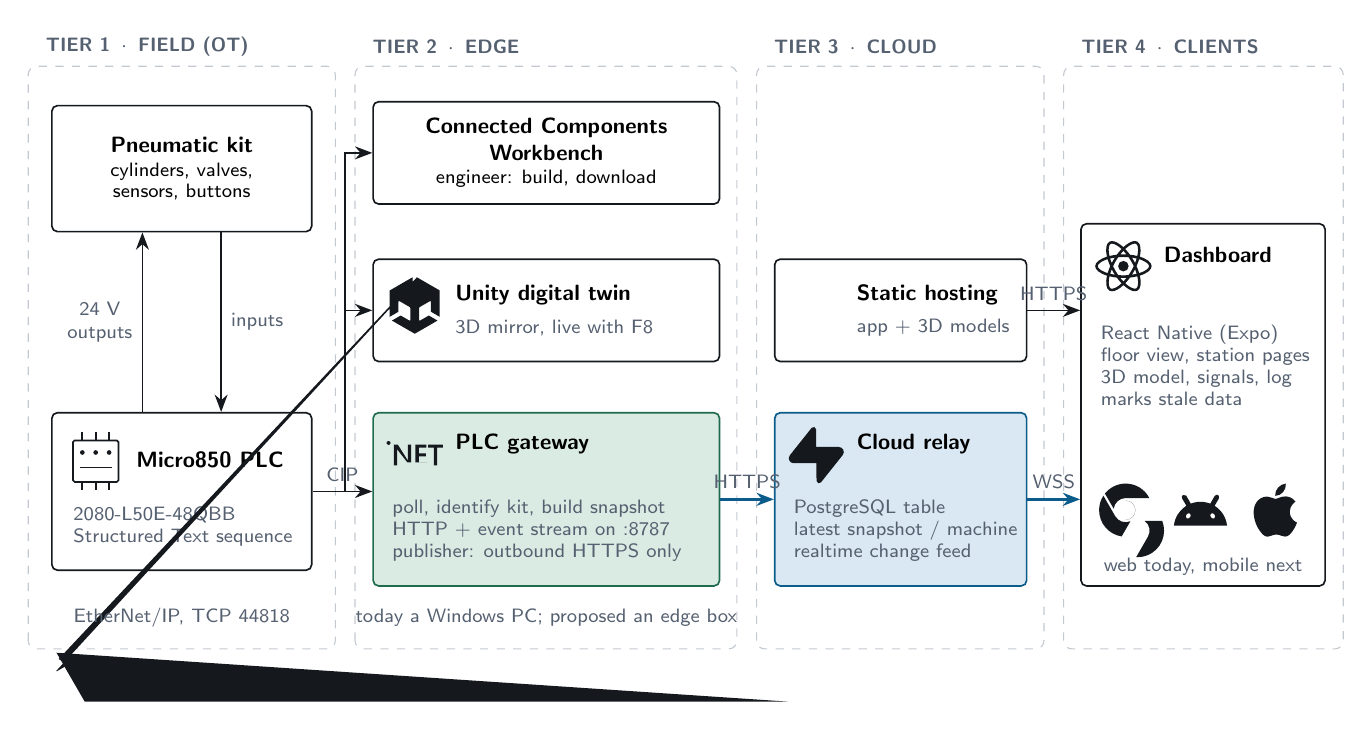
\begin{tikzpicture}[x=1cm,y=1cm]
  % lanes
  \draw[lane] (0,0) rectangle (3.9,7.4);   \node[hd,anchor=west] at (0.1,7.65) {TIER 1 \,$\cdot$\, FIELD (OT)};
  \draw[lane] (4.15,0) rectangle (9.0,7.4); \node[hd,anchor=west] at (4.25,7.65) {TIER 2 \,$\cdot$\, EDGE};
  \draw[lane] (9.25,0) rectangle (12.9,7.4);\node[hd,anchor=west] at (9.35,7.65) {TIER 3 \,$\cdot$\, CLOUD};
  \draw[lane] (13.15,0) rectangle (16.7,7.4);\node[hd,anchor=west] at (13.25,7.65) {TIER 4 \,$\cdot$\, CLIENTS};
  % field
  \node[box,minimum width=33mm,minimum height=16mm] (kit) at (1.95,6.1) {\textbf{Pneumatic kit}\\[-1pt]{\scriptsize cylinders, valves,}\\[-2pt]{\scriptsize sensors, buttons}};
  \node[box,minimum width=33mm,minimum height=20mm] (plc) at (1.95,2.0) {};
  \icoPlc{0.5}{2.75}{0.85}
  \node[anchor=west] at (1.25,2.4) {\textbf{Micro850 PLC}};
  \node[note,anchor=west,align=left] at (0.45,1.55) {2080-L50E-48QBB\\Structured Text sequence};
  \draw[wire] ([xshift=-5mm]plc.north) -- ([xshift=-5mm]kit.south) node[midway,left,note] {24 V\\outputs};
  \draw[wire] ([xshift=5mm]kit.south) -- ([xshift=5mm]plc.north) node[midway,right,note] {inputs};
  % edge
  \node[box,minimum width=44mm,minimum height=13mm] (ccw) at (6.58,6.3) {\textbf{Connected Components}\\\textbf{Workbench}\\[-1pt]{\scriptsize engineer: build, download}};
  \node[box,minimum width=44mm,minimum height=13mm] (unity) at (6.58,4.3) {};
  \icoUnity{4.55}{4.72}{0.85}\node[anchor=west] at (5.3,4.5) {\textbf{Unity digital twin}}; \node[note,anchor=west] at (5.3,4.08) {3D mirror, live with F8};
  \node[edgebox,minimum width=44mm,minimum height=22mm] (gw) at (6.58,1.9) {};
  \icoDotnet{4.55}{2.82}{0.85}\node[anchor=west] at (5.3,2.6) {\textbf{PLC gateway}};
  \node[note,anchor=west,align=left] at (4.5,1.5) {poll, identify kit, build snapshot\\HTTP + event stream on :8787\\publisher: outbound HTTPS only};
  \draw[wire] (plc.east) -- (gw.west |- plc.east) node[midway,above,note] {CIP};
  \draw[wire] (4.02,2.0) |- (unity.west);
  \draw[wire] (4.02,4.3) |- (ccw.west);
  \node[note] at (1.95,0.4) {EtherNet/IP, TCP 44818};
  \node[note] at (6.58,0.4) {today a Windows PC; proposed an edge box};
  % cloud
  \node[cloud,minimum width=32mm,minimum height=22mm] (relay) at (11.08,1.9) {};
  \icoSupabase{9.65}{2.82}{0.85}\node[anchor=west] at (10.4,2.6) {\textbf{Cloud relay}};
  \node[note,anchor=west,align=left] at (9.6,1.5) {PostgreSQL table\\latest snapshot / machine\\realtime change feed};
  \node[box,minimum width=32mm,minimum height=13mm] (host) at (11.08,4.3) {};
  \icoVercel{9.65}{4.72}{0.85}\node[anchor=west] at (10.4,4.5) {\textbf{Static hosting}}; \node[note,anchor=west] at (10.4,4.08) {app + 3D models};
  \draw[dwire] (gw.east |- relay.west) -- (relay.west) node[midway,above,note] {HTTPS};
  % clients
  \node[box,minimum width=31mm,minimum height=46mm] (app) at (14.92,3.1) {};
  \icoReact{13.55}{5.22}{0.85}\node[anchor=west] at (14.3,5.0) {\textbf{Dashboard}};
  \node[note,anchor=west,align=left] at (13.5,3.6) {React Native (Expo)\\floor view, station pages\\3D model, signals, log\\marks stale data};
  \icoGooglechrome{13.6}{2.1}{0.8}\icoAndroid{14.55}{2.1}{0.8}\icoApple{15.5}{2.1}{0.8}
  \node[note] at (14.92,1.05) {web today, mobile next};
  \draw[dwire] (relay.east) -- (app.west |- relay.east) node[midway,above,note] {WSS};
  \draw[wire] (host.east) -- (app.west |- host.east) node[midway,above,note] {HTTPS};
\end{tikzpicture}
\caption{High-level design as built. Blue arrows carry the published machine state. The engineering tool is the only component able to change the PLC program.}
\end{figure}

\subsection{Design decisions}
\begin{tabularx}{\textwidth}{@{}>{\raggedright\arraybackslash}p{42mm}YY@{}}
\toprule
\textbf{Decision} & \textbf{Reason} & \textbf{Consequence} \\
\midrule
Read the PLC by tag name over EtherNet/IP & Micro800 global variables are readable by name with no setup in the PLC project & No Modbus mapping to maintain; adding a signal is adding a name to a profile \\
Implement only the ``read tag'' service & A monitoring system must not be able to move a machine & Writing is impossible in this code path, not merely disabled \\
A gateway between the PLC and everything else & The PLC sits on a private link and changes its address & One place knows the protocol; twin, app and cloud consume plain JSON \\
Push from the plant to the cloud & No inbound firewall rule, no public address at the plant & The cloud holds the latest state and cannot reach back into the plant \\
Describe each machine in a profile file & Machines differ only in names, steps and labels & A new machine is a data file, not new code \\
\bottomrule
\end{tabularx}

% ------------------------------------------------------------------ 2
\section{Where each piece of software runs}

A common question is where the .NET gateway code actually executes. Today it runs on the \textbf{rig PC}: the
Windows computer on the bench that is plugged into the PLC. It is an ordinary console program, not a
service and not something inside the PLC or the cloud.

\begin{figure}[H]\centering
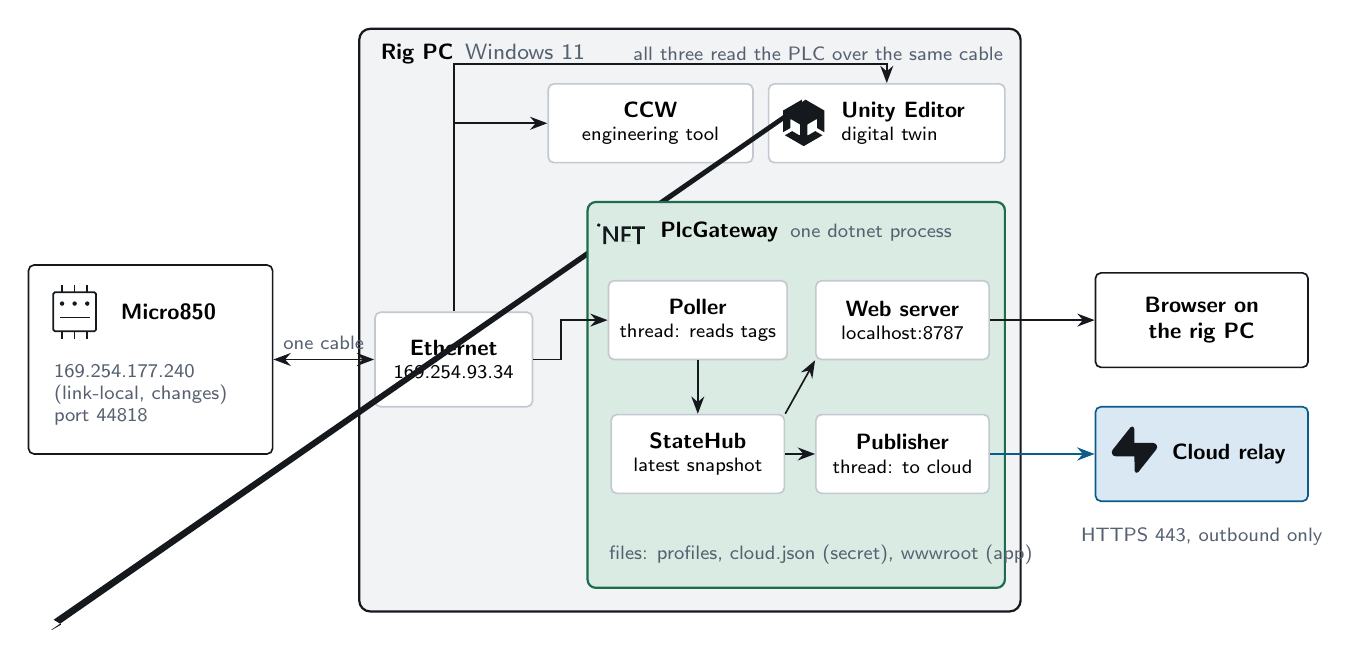
\begin{tikzpicture}[x=1cm,y=1cm]
  % the PLC
  \node[box,minimum width=31mm,minimum height=24mm] (plc) at (1.55,3.2) {};
  \icoPlc{0.25}{4.15}{0.8}\node[anchor=west] at (1.05,3.8) {\textbf{Micro850}};
  \node[note,anchor=west,align=left] at (0.2,2.75) {169.254.177.240\\(link-local, changes)\\port 44818};

  % the rig PC
  \draw[draw=ink,line width=0.8pt,rounded corners=4pt,fill=soft] (4.2,0) rectangle (12.6,7.4);
  \node[anchor=west] at (4.35,7.08) {\textbf{Rig PC} \,{\color{sub}Windows 11}};
  \node[subbox,minimum width=20mm,minimum height=12mm] (nic) at (5.4,3.2) {\textbf{Ethernet}\\[-1pt]{\scriptsize 169.254.93.34}};
  \node[subbox,minimum width=26mm,minimum height=10mm] (ccw) at (7.9,6.2) {\textbf{CCW}\\[-1pt]{\scriptsize engineering tool}};
  \node[subbox,minimum width=30mm,minimum height=10mm] (unity) at (10.9,6.2) {};
  \icoUnity{9.55}{6.5}{0.7}\node[anchor=west,align=left] at (10.2,6.2) {\textbf{Unity Editor}\\[-1pt]{\scriptsize digital twin}};

  % the gateway process
  \draw[draw=edge,line width=0.8pt,rounded corners=3pt,fill=edgesoft] (7.1,0.3) rectangle (12.4,5.2);
  \icoDotnet{7.22}{5.08}{0.72}
  \node[anchor=west] at (7.9,4.82) {\textbf{PlcGateway} \,{\color{sub}\scriptsize one dotnet process}};
  \node[subbox,minimum width=22mm,minimum height=10mm] (poll) at (8.5,3.7) {\textbf{Poller}\\[-1pt]{\scriptsize thread: reads tags}};
  \node[subbox,minimum width=22mm,minimum height=10mm] (hub) at (8.5,2.0) {\textbf{StateHub}\\[-1pt]{\scriptsize latest snapshot}};
  \node[subbox,minimum width=22mm,minimum height=10mm] (web) at (11.1,3.7) {\textbf{Web server}\\[-1pt]{\scriptsize localhost:8787}};
  \node[subbox,minimum width=22mm,minimum height=10mm] (pub) at (11.1,2.0) {\textbf{Publisher}\\[-1pt]{\scriptsize thread: to cloud}};
  \node[note,anchor=west] at (7.25,0.72) {files: profiles, cloud.json (secret), wwwroot (app)};
  \draw[wire] (poll) -- (hub);
  \draw[wire] (hub) -- (pub);
  \draw[wire] (hub.north east) -- (web.south west);

  % wiring
  \draw[wire,<->] (plc.east) -- (nic.west) node[midway,above,note] {one cable};
  \draw[wire] (nic.east) -- ++(0.35,0) |- (poll.west);
  \draw[wire] (nic.north) |- (ccw.west);
  \draw[wire] (nic.north |- ccw.west) -- ++(0,0.75) -| (unity.north);
  \node[note,anchor=east] at (12.5,7.08) {all three read the PLC over the same cable};

  % outside
  \node[box,minimum width=27mm,minimum height=12mm] (browser) at (14.9,3.7) {\textbf{Browser on}\\\textbf{the rig PC}};
  \node[cloud,minimum width=27mm,minimum height=12mm] (relay) at (14.9,2.0) {};
  \icoSupabase{13.75}{2.35}{0.7}\node[anchor=west] at (14.4,2.0) {\textbf{Cloud relay}};
  \draw[wire] (web.east) -- (browser.west);
  \draw[dwire] (pub.east) -- (relay.west);
  \node[note] at (14.9,0.95) {HTTPS 443, outbound only};
\end{tikzpicture}
\caption{Deployment today. The gateway is one process with two worker threads and a small web server. It is started by double-clicking \code{Tools/PlcGateway/start-gateway.cmd} (which runs \code{dotnet run}) and stops when that window is closed.}
\end{figure}

\begin{tabularx}{\textwidth}{@{}>{\raggedright\arraybackslash}p{36mm}>{\raggedright\arraybackslash}p{42mm}Y@{}}
\toprule
\textbf{Software} & \textbf{Runs on} & \textbf{Notes} \\
\midrule
PLC program (Structured Text) & Inside the Micro850 & Executes the machine sequence; unaware of the gateway \\
PLC gateway (.NET 10) & Rig PC, as a console process & Source in \code{Tools/PlcGateway}; needs the .NET runtime; must stay running for live data \\
Unity digital twin & Rig PC, Unity Editor & Reads the PLC directly with the same client; does not use the gateway \\
Cloud relay & Supabase (managed PostgreSQL) & Stores the latest snapshot per machine; no application code of ours runs here except one SQL function \\
Dashboard app & In the viewer's browser & Static files served by Vercel; all logic runs on the viewer's device \\
\bottomrule
\end{tabularx}

Because the gateway is plain .NET with no Windows-only dependency, the same code can run on Linux. That is
what makes the edge device in Section~\ref{sec:edge} a packaging change, not a rewrite.

% ------------------------------------------------------------------ 3
\section{How the PLC is read}

The controller speaks EtherNet/IP, which carries the Common Industrial Protocol (CIP). Reading one variable is
a CIP ``Read Tag'' request addressed by the variable's name. The gateway opens one connection and reuses it
for every read.

\begin{figure}[H]\centering
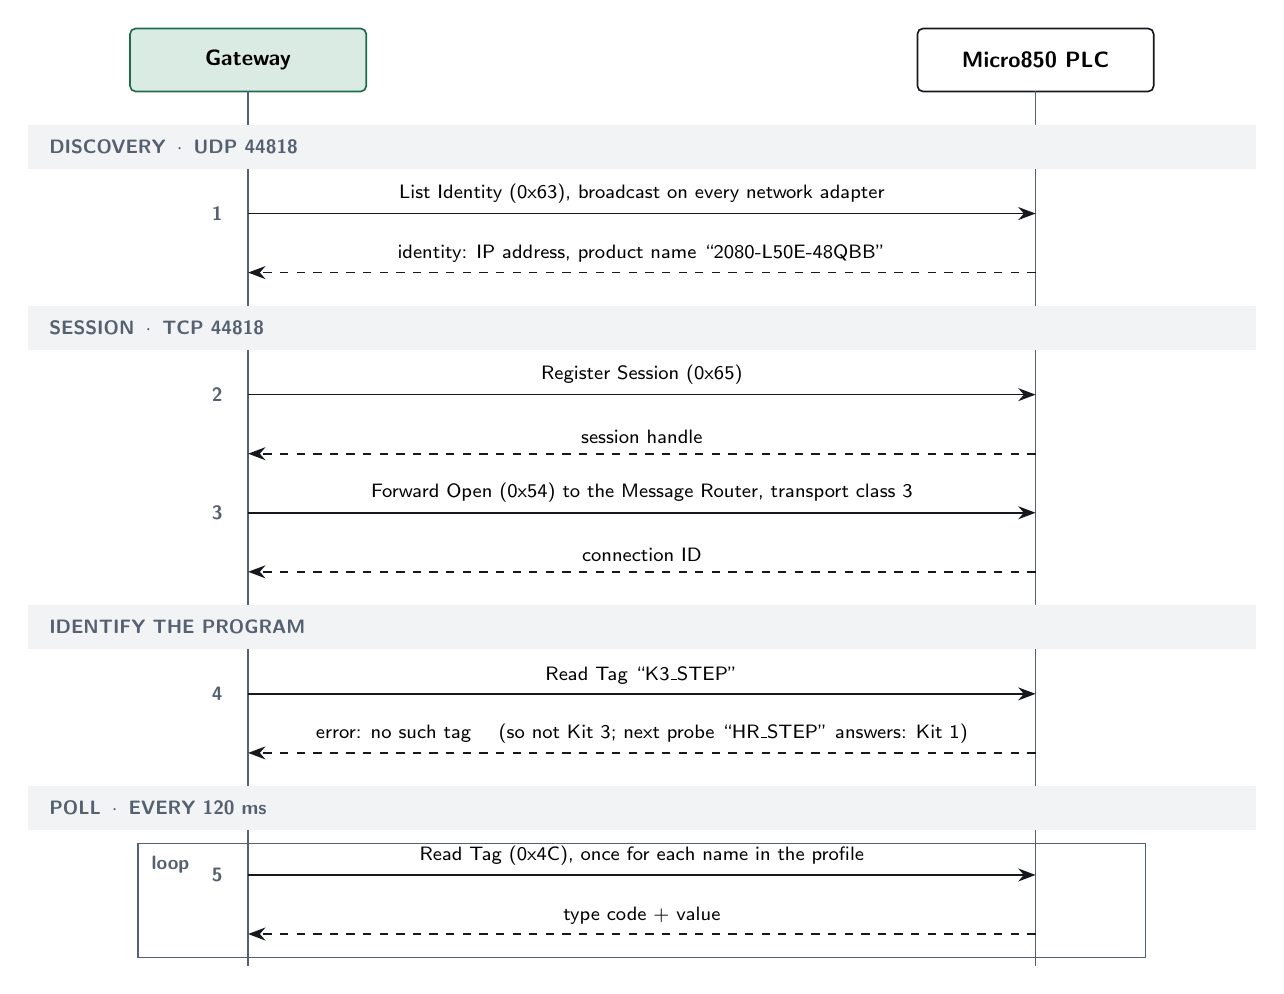
\begin{tikzpicture}[x=1cm,y=1cm]
  \node[edgebox,minimum width=30mm,minimum height=8mm] (g) at (3,0.6) {\textbf{Gateway}};
  \node[box,minimum width=30mm,minimum height=8mm] (p) at (13,0.6) {\textbf{Micro850 PLC}};
  \draw[line width=0.5pt,draw=sub] (3,0.2) -- (3,-10.9);
  \draw[line width=0.5pt,draw=sub] (13,0.2) -- (13,-10.9);
  \newcommand{\phase}[2]{\fill[soft] (0.2,#1+0.28) rectangle (15.8,#1-0.28); \node[hd,anchor=west] at (0.35,#1) {#2};}
  \newcommand{\req}[3]{\draw[wire] (3,#1) -- (13,#1) node[pos=0.5,above,font=\scriptsize] {#3}; \node[font=\scriptsize\bfseries,text=sub,anchor=east] at (2.8,#1) {#2};}
  \newcommand{\rsp}[2]{\draw[wire,dashed] (13,#1) -- (3,#1) node[pos=0.5,above,font=\scriptsize] {#2};}
  \phase{-0.5}{DISCOVERY \,$\cdot$\, UDP 44818}
  \req{-1.35}{1}{List Identity (0x63), broadcast on every network adapter}
  \rsp{-2.1}{identity: IP address, product name ``2080-L50E-48QBB''}
  \phase{-2.8}{SESSION \,$\cdot$\, TCP 44818}
  \req{-3.65}{2}{Register Session (0x65)}
  \rsp{-4.4}{session handle}
  \req{-5.15}{3}{Forward Open (0x54) to the Message Router, transport class 3}
  \rsp{-5.9}{connection ID}
  \phase{-6.6}{IDENTIFY THE PROGRAM}
  \req{-7.45}{4}{Read Tag ``K3\_STEP''}
  \rsp{-8.2}{error: no such tag \quad (so not Kit 3; next probe ``HR\_STEP'' answers: Kit 1)}
  \phase{-8.9}{POLL \,$\cdot$\, EVERY 120 ms}
  \req{-9.75}{5}{Read Tag (0x4C), once for each name in the profile}
  \rsp{-10.5}{type code + value}
  \draw[draw=sub,line width=0.5pt] (1.6,-9.35) rectangle (14.4,-10.8); \node[font=\scriptsize\bfseries,text=sub,anchor=north west] at (1.65,-9.38) {loop};
\end{tikzpicture}
\caption{Connecting and polling. The gateway finds the controller by broadcast because the PLC gives itself a new link-local address from time to time. It then binds its socket to the adapter that heard the reply, which avoids other adapters that share the same address range.}
\end{figure}

\begin{figure}[H]\centering
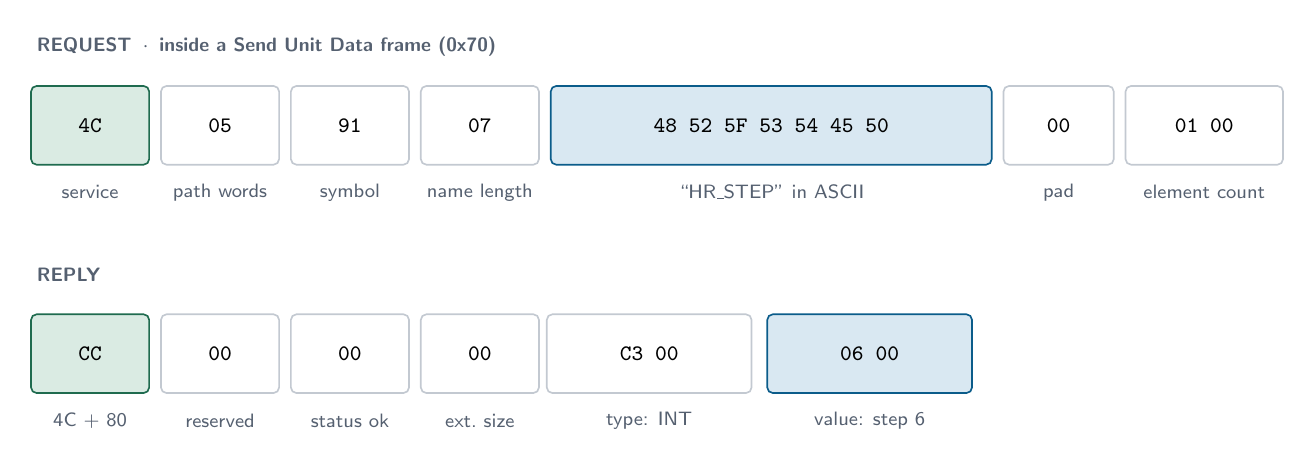
\begin{tikzpicture}[x=1cm,y=1cm]
  \newcommand{\byte}[5]{\node[#5,minimum width=#3,minimum height=10mm,inner sep=1pt] at (#1,#2) {\textbf{\ttfamily #4}};}
  \node[hd,anchor=west] at (0,1.0) {REQUEST \,$\cdot$\, inside a Send Unit Data frame (0x70)};
  \byte{0.8}{0}{15mm}{4C}{edgebox}        \node[note] at (0.8,-0.85) {service};
  \byte{2.45}{0}{15mm}{05}{subbox}        \node[note] at (2.45,-0.85) {path words};
  \byte{4.1}{0}{15mm}{91}{subbox}         \node[note] at (4.1,-0.85) {symbol};
  \byte{5.75}{0}{15mm}{07}{subbox}        \node[note] at (5.75,-0.85) {name length};
  \byte{9.45}{0}{56mm}{48 52 5F 53 54 45 50}{cloud} \node[note] at (9.45,-0.85) {``HR\_STEP'' in ASCII};
  \byte{13.1}{0}{14mm}{00}{subbox}        \node[note] at (13.1,-0.85) {pad};
  \byte{14.95}{0}{20mm}{01 00}{subbox}    \node[note] at (14.95,-0.85) {element count};
  \node[hd,anchor=west] at (0,-1.9) {REPLY};
  \byte{0.8}{-2.9}{15mm}{CC}{edgebox}     \node[note] at (0.8,-3.75) {4C + 80};
  \byte{2.45}{-2.9}{15mm}{00}{subbox}     \node[note] at (2.45,-3.75) {reserved};
  \byte{4.1}{-2.9}{15mm}{00}{subbox}      \node[note] at (4.1,-3.75) {status ok};
  \byte{5.75}{-2.9}{15mm}{00}{subbox}     \node[note] at (5.75,-3.75) {ext.\ size};
  \byte{7.9}{-2.9}{26mm}{C3 00}{subbox}   \node[note] at (7.9,-3.75) {type: INT};
  \byte{10.7}{-2.9}{26mm}{06 00}{cloud}   \node[note] at (10.7,-3.75) {value: step 6};
\end{tikzpicture}
\caption{A Read Tag request and reply, byte by byte. Names are matched without regard to case. Type codes handled: C1 BOOL, C2 SINT, C3 INT, C4 DINT (also TIME, in milliseconds), C6 to C8 unsigned.}
\end{figure}

\begin{minipage}[t]{0.53\textwidth}
\subsection{What is read}
\begin{tabularx}{\linewidth}{@{}lY@{}}
\toprule
\textbf{Group} & \textbf{Example tags} \\
\midrule
Sequence & \code{HR\_STEP}, \code{HR\_FAULTCODE} \\
Status & \code{ST\_AUTORUNNING}, \code{ST\_FAULTED} \\
Counters & \code{HR\_PARTSDONE}, \code{HR\_METALCOUNT} \\
Raw inputs & \code{\_IO\_EM\_DI\_00} \dots\ \code{\_IO\_EM\_DI\_13} \\
Raw outputs & \code{\_IO\_EM\_DO\_00} \dots\ \code{\_IO\_EM\_DO\_07} \\
Settings & \code{CFG\_TRAVELTIME}, \code{CFG\_MOVETIMEOUT} \\
\bottomrule
\end{tabularx}
\end{minipage}\hfill
\begin{minipage}[t]{0.43\textwidth}
\subsection{Time budget of one poll}
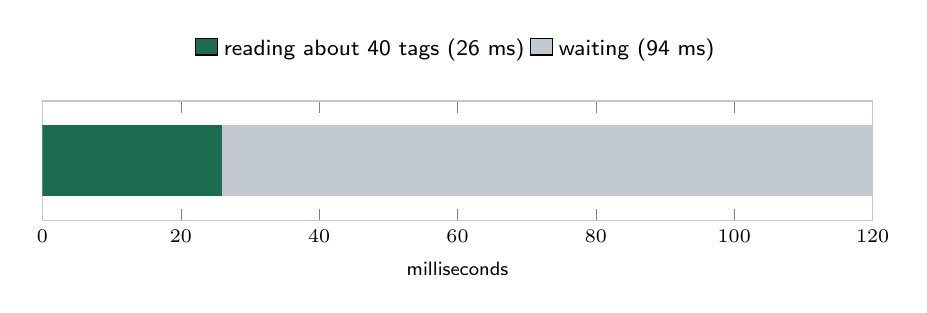
\begin{tikzpicture}
\begin{axis}[xbar stacked,width=\linewidth,height=3.1cm,xmin=0,xmax=120,ytick=\empty,
  xlabel={milliseconds},xlabel style={font=\scriptsize},tick label style={font=\scriptsize},
  axis line style={draw=rule},bar width=9mm,enlarge y limits=0.6,
  legend style={at={(0.5,1.25)},anchor=south,legend columns=2,draw=none,font=\scriptsize}]
  \addplot[fill=edge,draw=none] coordinates {(26,0)};
  \addplot[fill=rule,draw=none] coordinates {(94,0)};
  \legend{reading about 40 tags (26 ms), waiting (94 ms)}
\end{axis}
\end{tikzpicture}

{\small\color{sub}One tag read takes about 0.65 ms; a full scan was measured at 24 to 28 ms.}
\end{minipage}

\medskip
Tags are read one per request. The protocol also allows several reads in one frame (the Multiple Service
Packet); that is not implemented, and at 26 ms for a full scan it has not been needed.

% ------------------------------------------------------------------ 4
\section{Low-level design}

\subsection{Gateway components}
\begin{figure}[H]\centering
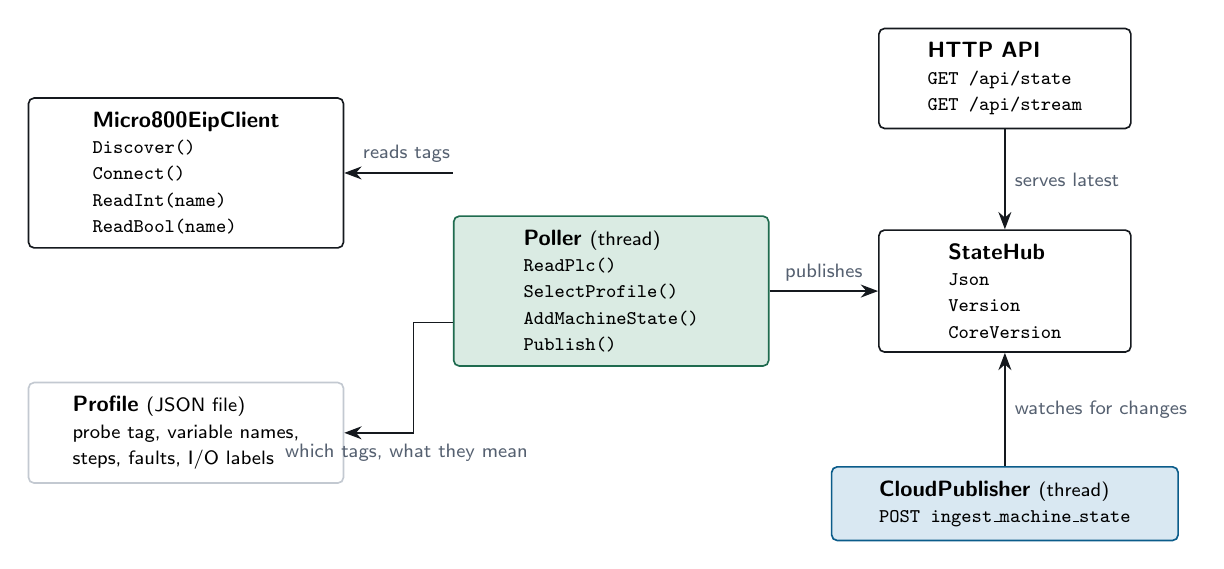
\begin{tikzpicture}[x=1cm,y=1cm]
  \newcommand{\cls}[5]{\node[#5,minimum width=#4,align=left,inner sep=5pt] (#1) at #2 {#3};}
  \cls{eip}{(2.2,3.9)}{\textbf{Micro800EipClient}\\{\scriptsize\ttfamily Discover()}\\{\scriptsize\ttfamily Connect()}\\{\scriptsize\ttfamily ReadInt(name)}\\{\scriptsize\ttfamily ReadBool(name)}}{40mm}{box}
  \cls{prof}{(2.2,0.6)}{\textbf{Profile} {\scriptsize(JSON file)}\\{\scriptsize probe tag, variable names,}\\{\scriptsize steps, faults, I/O labels}}{40mm}{subbox}
  \cls{poll}{(7.6,2.4)}{\textbf{Poller} {\scriptsize(thread)}\\{\scriptsize\ttfamily ReadPlc()}\\{\scriptsize\ttfamily SelectProfile()}\\{\scriptsize\ttfamily AddMachineState()}\\{\scriptsize\ttfamily Publish()}}{40mm}{edgebox}
  \cls{hub}{(12.6,2.4)}{\textbf{StateHub}\\{\scriptsize\ttfamily Json}\\{\scriptsize\ttfamily Version}\\{\scriptsize\ttfamily CoreVersion}}{32mm}{box}
  \cls{api}{(12.6,5.1)}{\textbf{HTTP API}\\{\scriptsize\ttfamily GET /api/state}\\{\scriptsize\ttfamily GET /api/stream}}{32mm}{box}
  \cls{pub}{(12.6,-0.3)}{\textbf{CloudPublisher} {\scriptsize(thread)}\\{\scriptsize\ttfamily POST ingest\_machine\_state}}{44mm}{cloud}
  \draw[wire] (poll.west |- eip.east) -- ++(-0.5,0) |- (eip.east);
  \node[note] at (5.0,4.15) {reads tags};
  \draw[wire] ([yshift=-4mm]poll.west) -- ++(-0.5,0) |- (prof.east);
  \node[note] at (5.0,0.35) {which tags, what they mean};
  \draw[wire] (poll) -- (hub) node[midway,above,note] {publishes};
  \draw[wire] (api) -- (hub) node[midway,right,note] {serves latest};
  \draw[wire] (pub) -- (hub) node[midway,right,note] {watches for changes};
\end{tikzpicture}
\caption{The gateway's parts. The poller and the cloud publisher are background threads; they share only the StateHub, which holds the latest snapshot as text and two version counters.}
\end{figure}

\subsection{Poll loop}
\begin{figure}[H]\centering
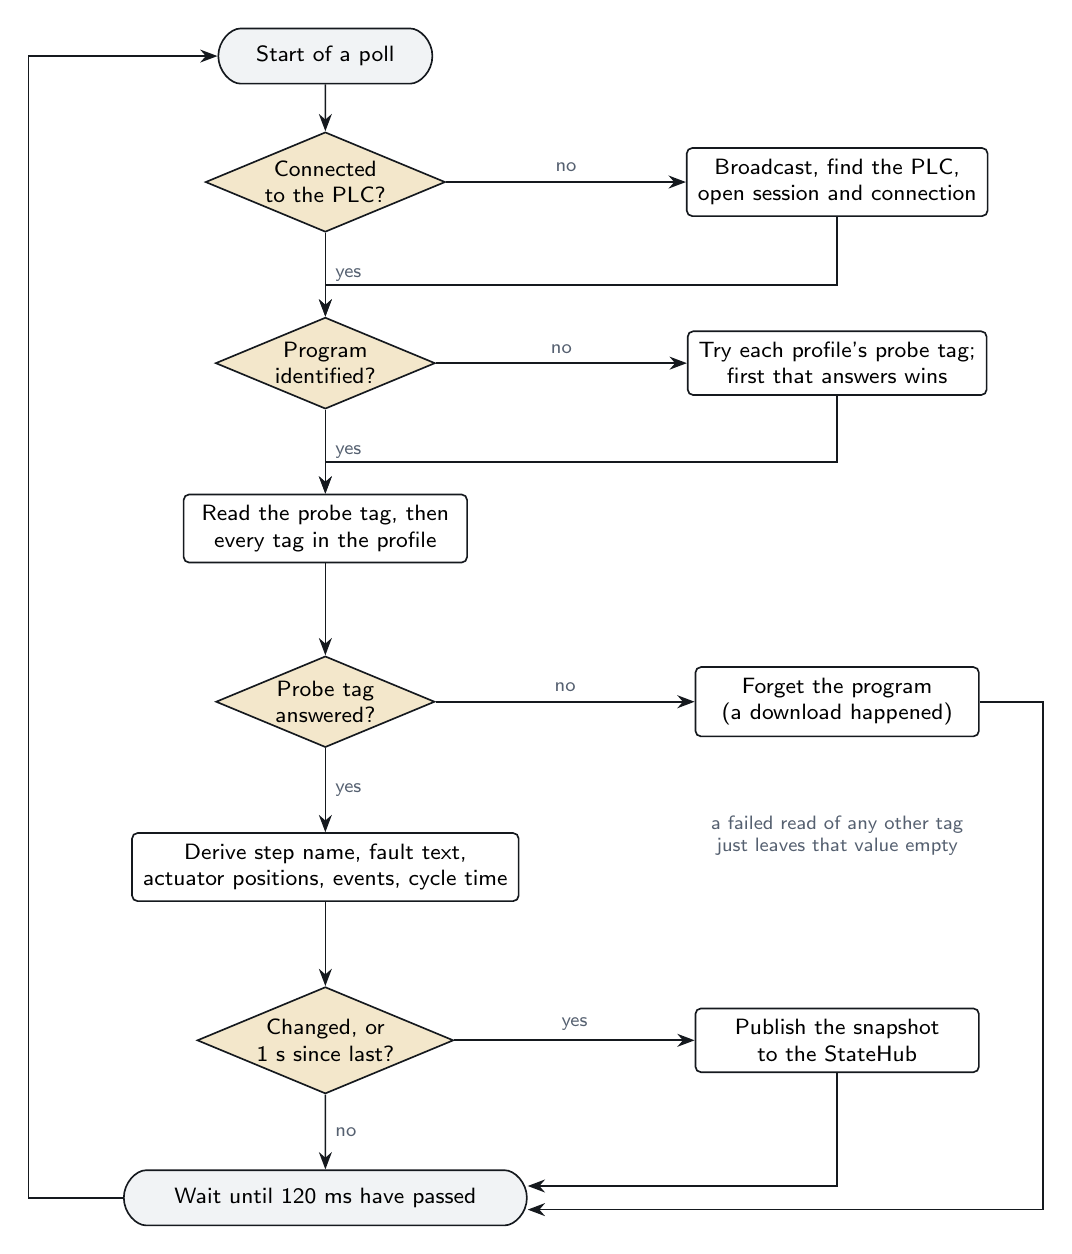
\begin{tikzpicture}[x=1cm,y=1cm,node distance=6mm]
  \node[term] (start) at (4,0) {Start of a poll};
  \node[dec] (conn) at (4,-1.6) {Connected\\to the PLC?};
  \node[proc] (disc) at (10.5,-1.6) {Broadcast, find the PLC,\\open session and connection};
  \node[dec] (known) at (4,-3.9) {Program\\identified?};
  \node[proc] (probe) at (10.5,-3.9) {Try each profile's probe tag;\\first that answers wins};
  \node[proc] (read) at (4,-6.0) {Read the probe tag, then\\every tag in the profile};
  \node[dec] (ok) at (4,-8.2) {Probe tag\\answered?};
  \node[proc] (forget) at (10.5,-8.2) {Forget the program\\(a download happened)};
  \node[proc] (derive) at (4,-10.3) {Derive step name, fault text,\\actuator positions, events, cycle time};
  \node[dec] (chg) at (4,-12.5) {Changed, or\\1 s since last?};
  \node[proc] (pubn) at (10.5,-12.5) {Publish the snapshot\\to the StateHub};
  \node[term,minimum width=54mm] (wait) at (4,-14.5) {Wait until 120 ms have passed};
  \draw[wire] (start) -- (conn);
  \draw[wire] (conn) -- node[above,note] {no} (disc);
  \draw[wire] (conn) -- node[right,note] {yes} (known);
  \draw[wire] (disc) |- ([yshift=4mm]known.north) -- (known.north);
  \draw[wire] (known) -- node[above,note] {no} (probe);
  \draw[wire] (known) -- node[right,note] {yes} (read);
  \draw[wire] (probe) |- ([yshift=4mm]read.north) -- (read.north);
  \draw[wire] (read) -- (ok);
  \draw[wire] (ok) -- node[above,note] {no} (forget);
  \draw[wire] (ok) -- node[right,note] {yes} (derive);
  \draw[wire] (derive) -- (chg);
  \draw[wire] (chg) -- node[above,note] {yes} (pubn);
  \draw[wire] (chg) -- node[right,note] {no} (wait);
  \draw[wire] (pubn.south) |- ([yshift=1.5mm]wait.east);
  \draw[wire] (forget.east) -- ++(0.8,0) |- ([yshift=-1.5mm]wait.east);
  \draw[wire] (wait.west) -- ++(-1.2,0) |- (start.west);
  \node[note,align=center] at (10.5,-9.9) {a failed read of any other tag\\just leaves that value empty};
\end{tikzpicture}
\caption{Flowchart of one poll. A connection error anywhere jumps to ``not connected'' and the loop waits 2 s before trying again.}
\end{figure}

\subsection{What the gateway adds to the raw values}
\begin{itemize}
  \item \textbf{Meaning.} Step 6 becomes ``Upper eject''; fault 9 becomes ``Homing did not finish''.
  \item \textbf{Actuator position.} Worked out from the two valve coils. With neither coil on, the last commanded position is kept, because these valves hold their place.
  \item \textbf{Events.} A rolling log of step changes, faults, parts counted and link changes.
  \item \textbf{Cycle time.} From the feed step to the part counter increasing.
\end{itemize}

\subsection{Snapshot contract}
Every consumer receives the same document. It is self-describing: labels and step names travel with the
values, so the app needs no knowledge of a particular machine.
\begin{lstlisting}
{
  "ts": "2026-11-18T10:25:32.444Z",
  "gateway": { "version": "0.1.0", "mode": "plc", "readOnly": true },
  "link":    { "connected": true, "plc": "169.254.177.240", "product": "2080-L50E-48QBB", "readMs": 24 },
  "kit":     { "id": "kit1", "name": "Kit 1", "steps": [ { "id": 6, "name": "Upper eject" } ] },
  "status":  { "state": "fault", "step": 90, "faultCode": 9, "faultText": "Homing did not finish" },
  "counters":  [ { "id": "parts", "label": "Parts sorted", "value": 0 } ],
  "inputs":    [ { "id": "DI-2", "label": "2A pulled in", "on": false } ],
  "outputs":   [ { "id": "DO-6", "label": "Lift up", "on": false } ],
  "actuators": [ { "id": "4A", "label": "Lift", "positionLabel": "Up", "driven": false } ],
  "cycle":   { "lastSeconds": null, "averageSeconds": null, "history": [] },
  "events":  [ { "ts": "...", "kind": "fault", "text": "Fault 9 - Homing did not finish" } ]
}
\end{lstlisting}

\subsection{Interfaces}
\begin{tabularx}{\textwidth}{@{}>{\raggedright\arraybackslash}p{37mm}>{\raggedright\arraybackslash}p{33mm}>{\raggedright\arraybackslash}p{38mm}Y@{}}
\toprule
\textbf{Interface} & \textbf{Direction} & \textbf{Protocol} & \textbf{Notes} \\
\midrule
PLC and gateway & Gateway asks & EtherNet/IP, UDP + TCP 44818 & Read Tag only \\
\code{GET /api/state} & Local consumers pull & HTTP, port 8787 & Latest snapshot \\
\code{GET /api/stream} & Gateway pushes & Server-Sent Events & On change; keep-alive every 15 s \\
Any other HTTP method & -- & -- & Refused with status 405 \\
Gateway to relay & Outbound only & HTTPS, port 443 & \code{rpc/ingest\_machine\_state}; token checked \\
Relay to app & App subscribes & Secure WebSocket, 443 & Row changes; a 10 s re-read as a safety net \\
PLC and Unity twin & Twin asks & EtherNet/IP & Same read-only client, own thread \\
\bottomrule
\end{tabularx}

\subsection{Publishing to the cloud}
\begin{figure}[H]\centering
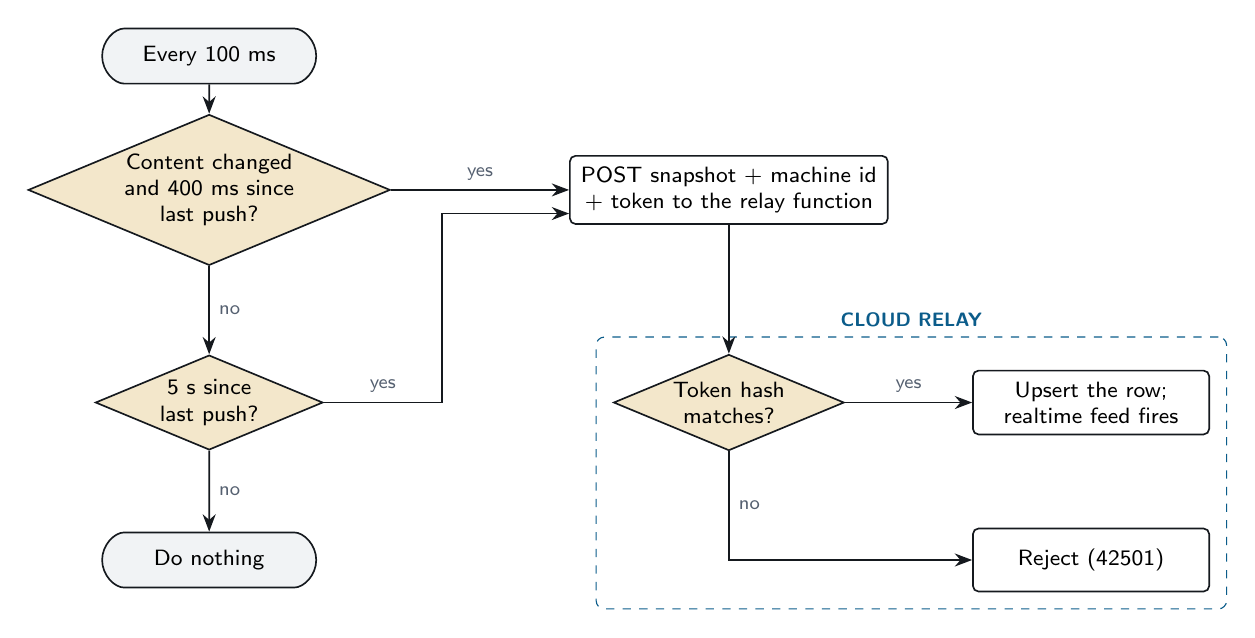
\begin{tikzpicture}[x=1cm,y=1cm]
  \node[term] (s) at (3.2,0) {Every 100 ms};
  \node[dec] (c) at (3.2,-1.7) {Content changed\\and 400 ms since\\last push?};
  \node[dec] (h) at (3.2,-4.4) {5 s since\\last push?};
  \node[proc] (p) at (9.8,-1.7) {POST snapshot + machine id\\+ token to the relay function};
  \node[dec] (t) at (9.8,-4.4) {Token hash\\matches?};
  \node[proc,minimum width=30mm] (u) at (14.4,-4.4) {Upsert the row;\\realtime feed fires};
  \node[proc,minimum width=30mm] (r) at (14.4,-6.4) {Reject (42501)};
  \node[term] (e) at (3.2,-6.4) {Do nothing};
  \draw[wire] (s) -- (c);
  \draw[wire] (c) -- node[above,note] {yes} (p);
  \draw[wire] (c) -- node[right,note] {no} (h);
  \draw[wire] (h) -- node[right,note] {no} (e);
  \draw[wire] (h.east) -- node[above,note] {yes} ++(1.5,0) |- ([yshift=-3mm]p.west);
  \draw[wire] (p) -- (t);
  \draw[wire] (t) -- node[above,note] {yes} (u);
  \draw[wire] (t.south) |- node[pos=0.25,right,note] {no} (r.west);
  \begin{scope}[on background layer]
    \node[draw=data,dashed,rounded corners=3pt,fit=(t)(u)(r),inner sep=6pt,label={[font=\scriptsize\bfseries,text=data]above:CLOUD RELAY}] {};
  \end{scope}
\end{tikzpicture}
\caption{Flowchart of the cloud publisher (left, on the rig PC) and the relay's check (right, in the database). Publishing is throttled to one push per 400 ms while values change and one every 5 s when nothing does.}
\end{figure}

\begin{tabularx}{\textwidth}{@{}>{\raggedright\arraybackslash}p{46mm}YY@{}}
\toprule
\textbf{Relay object} & \textbf{Purpose} & \textbf{Access} \\
\midrule
\code{machine\_state} (table) & One row per machine: id, snapshot, updated\_at & Anyone may read; nobody may write directly \\
\code{machine\_ingest\_keys} (table) & SHA-256 of each machine's token & No access through the API \\
\code{ingest\_machine\_state()} & Checks the token, then upserts the row & Callable with the public key \\
\bottomrule
\end{tabularx}

\subsection{Freshness in the app}
\begin{figure}[H]\centering
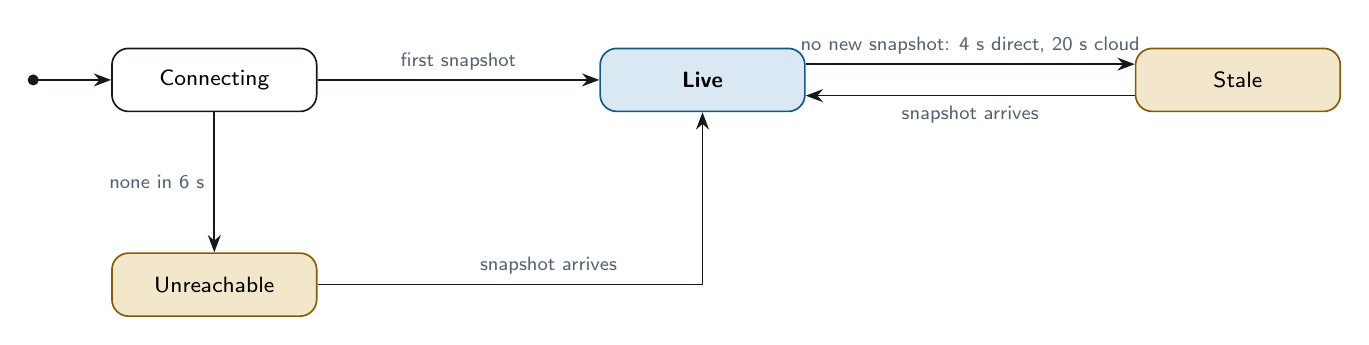
\begin{tikzpicture}[x=1cm,y=1cm]
  \node[state] (c) at (0,0) {Connecting};
  \node[state,draw=data,fill=datasoft] (l) at (6.2,0) {\textbf{Live}};
  \node[state,draw=warn,fill=warnsoft] (s) at (13.0,0) {Stale};
  \node[state,draw=warn,fill=warnsoft] (u) at (0,-2.6) {Unreachable};
  \fill[ink] (-2.3,0) circle (2pt);
  \draw[wire] (-2.3,0) -- (c);
  \draw[wire] (c) -- node[above,note] {first snapshot} (l);
  \draw[wire] (c) -- node[left,note] {none in 6 s} (u);
  \draw[wire] (u) -| node[pos=0.3,above,note] {snapshot arrives} (l);
  \draw[wire] ([yshift=2mm]l.east) -- node[above,note] {no new snapshot: 4 s direct, 20 s cloud} ([yshift=2mm]s.west);
  \draw[wire] ([yshift=-2mm]s.west) -- node[below,note] {snapshot arrives} ([yshift=-2mm]l.east);
\end{tikzpicture}
\caption{The app's view of data freshness. ``Stale'' dims the values and labels them ``last known''. The app never presents an old reading as current.}
\end{figure}

\subsection{Digital twin link}
The Unity twin uses the same EtherNet/IP client on its own thread and reads the PLC directly; it does not go
through the gateway. While the link is live, the twin's own sequencer and manual controls are switched off,
its cylinders follow the real solenoid outputs, and the workpiece is coloured once the real sensors classify
it. If the link drops, the twin returns to offline simulation.

% ------------------------------------------------------------------ 5
\section{Proposal: a compact edge device}\label{sec:edge}

Today the ``edge'' is a Windows PC on the bench. It works, but it is large, it is someone's workstation, and
it sends far more data than it needs to. A small dedicated device fixes all three. \textbf{Everything in this
section is a proposal; none of it is built yet.}

\begin{figure}[H]\centering
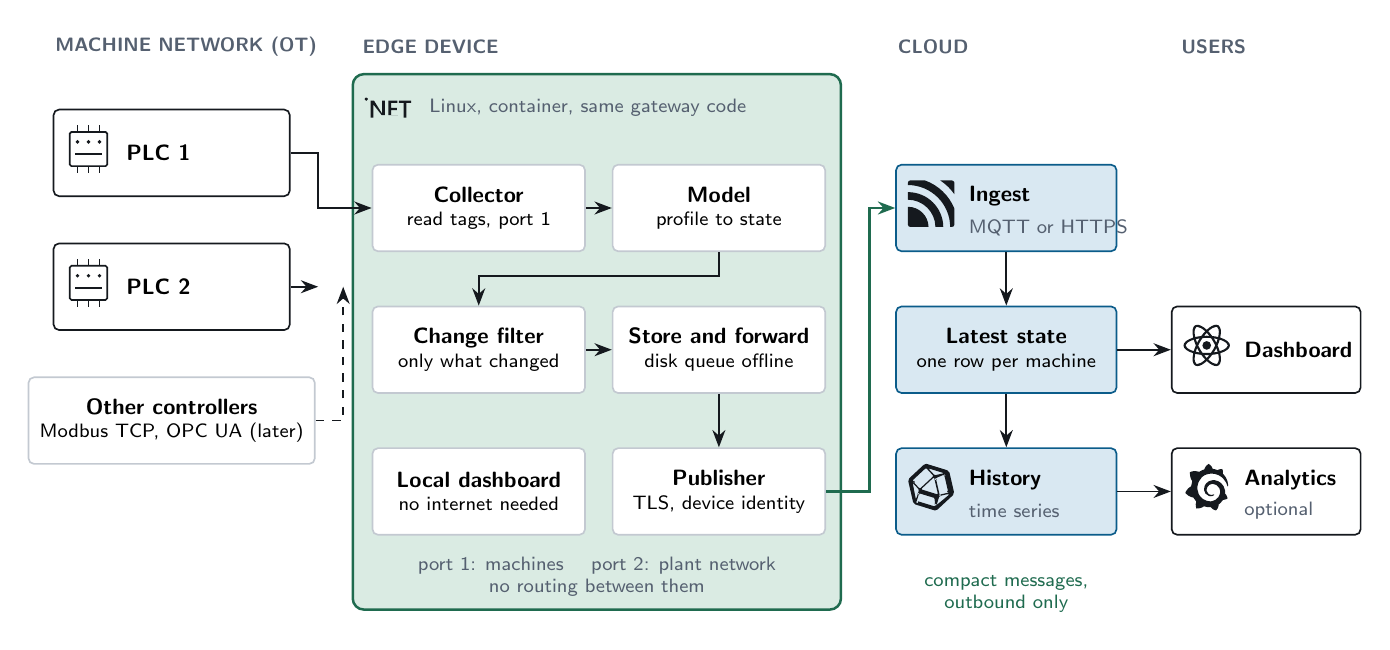
\begin{tikzpicture}[x=1cm,y=1cm]
  \node[hd,anchor=west] at (0,7.75) {MACHINE NETWORK (OT)}; \node[hd,anchor=west] at (3.9,7.75) {EDGE DEVICE}; \node[hd,anchor=west] at (10.7,7.75) {CLOUD}; \node[hd,anchor=west] at (14.3,7.75) {USERS};
  \node[box,minimum width=30mm,minimum height=11mm] (p1) at (1.6,6.4) {};
  \icoPlc{0.25}{6.75}{0.7}\node[anchor=west] at (0.9,6.4) {\textbf{PLC 1}};
  \node[box,minimum width=30mm,minimum height=11mm] (p2) at (1.6,4.7) {};
  \icoPlc{0.25}{5.05}{0.7}\node[anchor=west] at (0.9,4.7) {\textbf{PLC 2}};
  \node[subbox,minimum width=30mm,minimum height=11mm] (p3) at (1.6,3.0) {\textbf{Other controllers}\\[-1pt]{\scriptsize Modbus TCP, OPC UA (later)}};

  \draw[draw=edge,line width=0.9pt,rounded corners=4pt,fill=edgesoft] (3.9,0.6) rectangle (10.1,7.4);
  \icoDotnet{4.05}{7.25}{0.7}
  \node[note,anchor=west] at (4.75,6.98) {Linux, container, same gateway code};
  \node[subbox,minimum width=27mm,minimum height=11mm] (col) at (5.5,5.7) {\textbf{Collector}\\[-1pt]{\scriptsize read tags, port 1}};
  \node[subbox,minimum width=27mm,minimum height=11mm] (mod) at (8.55,5.7) {\textbf{Model}\\[-1pt]{\scriptsize profile to state}};
  \node[subbox,minimum width=27mm,minimum height=11mm] (flt) at (5.5,3.9) {\textbf{Change filter}\\[-1pt]{\scriptsize only what changed}};
  \node[subbox,minimum width=27mm,minimum height=11mm] (buf) at (8.55,3.9) {\textbf{Store and forward}\\[-1pt]{\scriptsize disk queue offline}};
  \node[subbox,minimum width=27mm,minimum height=11mm] (loc) at (5.5,2.1) {\textbf{Local dashboard}\\[-1pt]{\scriptsize no internet needed}};
  \node[subbox,minimum width=27mm,minimum height=11mm] (pub) at (8.55,2.1) {\textbf{Publisher}\\[-1pt]{\scriptsize TLS, device identity}};
  \draw[wire] (col) -- (mod); \draw[wire] (mod.south) -- ++(0,-0.3) -| (flt.north); \draw[wire] (flt) -- (buf); \draw[wire] (buf) -- (pub);
  \node[note] at (7.0,1.02) {port 1: machines \quad port 2: plant network\\no routing between them};
  \draw[wire] (p1.east) -- ++(0.35,0) |- (col.west);
  \draw[wire] (p2.east) -- ++(0.35,0);
  \draw[wire,dashed] (p3.east) -- ++(0.35,0) -- ++(0,1.7);

  \node[cloud,minimum width=28mm,minimum height=11mm] (ing) at (12.2,5.7) {};
  \icoMqtt{10.95}{6.05}{0.7}\node[anchor=west] at (11.6,5.85) {\textbf{Ingest}}; \node[note,anchor=west] at (11.6,5.45) {MQTT or HTTPS};
  \node[cloud,minimum width=28mm,minimum height=11mm] (lat) at (12.2,3.9) {\textbf{Latest state}\\[-1pt]{\scriptsize one row per machine}};
  \node[cloud,minimum width=28mm,minimum height=11mm] (his) at (12.2,2.1) {};
  \icoInfluxdb{10.95}{2.45}{0.7}\node[anchor=west] at (11.6,2.25) {\textbf{History}}; \node[note,anchor=west] at (11.6,1.85) {time series};
  \draw[ewire] (pub.east) -- ++(0.55,0) |- (ing.west);
  \node[note,text=edge] at (12.2,0.8) {compact messages,\\outbound only};
  \draw[wire] (ing) -- (lat); \draw[wire] (lat) -- (his);

  \node[box,minimum width=24mm,minimum height=11mm] (dash) at (15.5,3.9) {};
  \icoReact{14.45}{4.25}{0.7}\node[anchor=west] at (15.1,3.9) {\textbf{Dashboard}};
  \node[box,minimum width=24mm,minimum height=11mm] (an) at (15.5,2.1) {};
  \icoGrafana{14.45}{2.45}{0.7}\node[anchor=west] at (15.1,2.25) {\textbf{Analytics}}; \node[note,anchor=west] at (15.1,1.85) {optional};
  \draw[wire] (lat) -- (dash); \draw[wire] (his) -- (an);
\end{tikzpicture}
\caption{Proposed high-level design with an edge device (green is new). The cloud side adds a history store, which the current system does not have: today only the latest state is kept.}
\end{figure}

\subsection{Making the data compact}
The gateway currently sends the whole self-describing snapshot every time: about 5 kB, of which almost all
is labels, step names and an event log that did not change. Four steps shrink it.
\begin{enumerate}
  \item \textbf{Send the description once.} Labels, step names and fault texts are static. Publish the profile when it changes and refer to it by version afterwards.
  \item \textbf{Report by exception.} Send a value only when it changes, plus a heartbeat so the cloud knows the device is alive.
  \item \textbf{Pack the bits.} Kit 1's 22 inputs and outputs fit in 3 bytes. With step, fault, material, three counters and a timestamp, a full state frame is 17 bytes.
  \item \textbf{Batch and compress when the link is poor.} Group several frames into one message.
\end{enumerate}

\begin{figure}[H]\centering
\begin{minipage}{0.56\textwidth}\centering
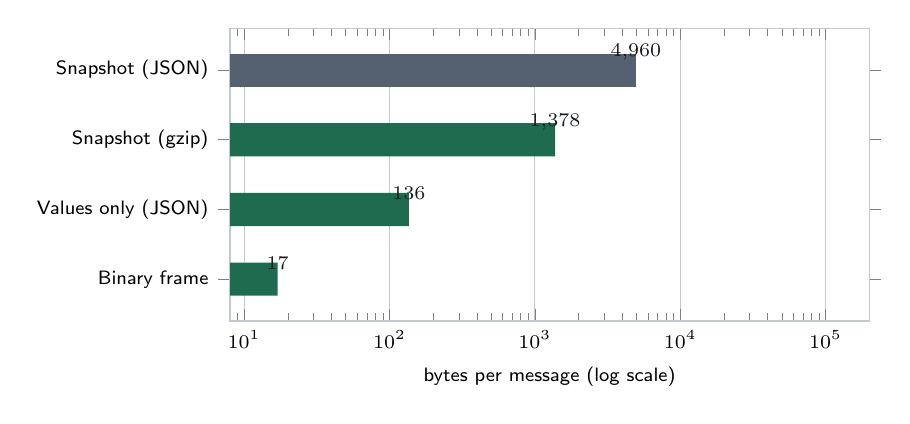
\begin{tikzpicture}
\begin{axis}[xbar,xmode=log,width=0.8\linewidth,height=5.3cm,xmin=8,xmax=200000,
  ytick={1,2,3,4},yticklabels={Binary frame,Values only (JSON),Snapshot (gzip),Snapshot (JSON)},
  tick label style={font=\scriptsize},xlabel={bytes per message (log scale)},xlabel style={font=\scriptsize},
  nodes near coords,nodes near coords style={font=\scriptsize,text=ink},point meta=rawx,
  axis line style={draw=rule},bar width=4.2mm,bar shift=0pt,log origin=infty,enlarge y limits=0.2,xmajorgrids,grid style={draw=rule}]
  \addplot[fill=edge,draw=none] coordinates {(17,1) (136,2) (1378,3)};
  \addplot[fill=sub,draw=none,bar shift=0pt] coordinates {(4960,4)};
\end{axis}
\end{tikzpicture}
\end{minipage}\hfill
\begin{minipage}{0.42\textwidth}\centering
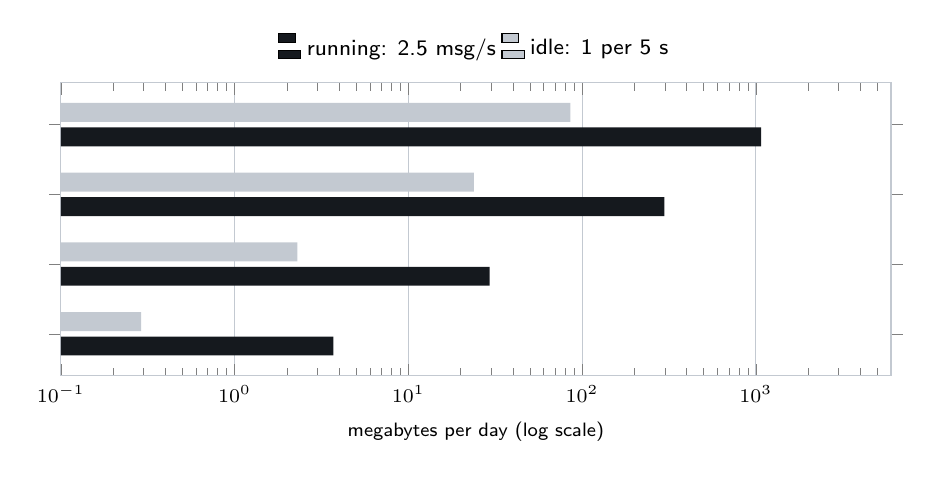
\begin{tikzpicture}
\begin{axis}[xbar,xmode=log,log origin=infty,width=\linewidth,height=5.3cm,xmin=0.1,xmax=6000,
  ytick={1,2,3,4},yticklabels={},
  tick label style={font=\scriptsize},xlabel={megabytes per day (log scale)},xlabel style={font=\scriptsize},
  axis line style={draw=rule},bar width=2.4mm,enlarge y limits=0.2,xmajorgrids,grid style={draw=rule},
  legend style={at={(0.5,1.04)},anchor=south,legend columns=2,font=\scriptsize,draw=none}]
  \addplot[fill=ink,draw=none] coordinates {(3.7,1) (29.4,2) (298,3) (1071,4)};
  \addplot[fill=rule,draw=none] coordinates {(0.29,1) (2.3,2) (23.8,3) (85.7,4)};
  \legend{running: 2.5 msg/s, idle: 1 per 5 s}
\end{axis}
\end{tikzpicture}
\end{minipage}
\caption{Left: bytes per state message for Kit 1. The three larger values were measured on the running gateway on 18 November 2026; the binary frame is calculated from the field list above. Right: resulting payload per day, calculated from those sizes and the configured publish rates, without protocol overhead.}
\end{figure}

\begin{tabularx}{\textwidth}{@{}Yrrrl@{}}
\toprule
\textbf{Encoding} & \textbf{Bytes / message} & \textbf{MB / day running} & \textbf{MB / day idle} & \textbf{Basis} \\
\midrule
Full snapshot, JSON (today) & 4,960 & 1,071 & 85.7 & measured size \\
Full snapshot, gzip & 1,378 & 298 & 23.8 & measured size \\
Values only, JSON & 136 & 29.4 & 2.3 & measured size \\
Values only, binary frame & 17 & 3.7 & 0.29 & calculated \\
\bottomrule
\end{tabularx}

The ``running'' column assumes the machine changes state at the maximum publish rate all day, which is a
ceiling. The point is the ratio: about 290 times less data, which is the difference between needing a wired
connection and running comfortably on a cellular modem.

\subsection{What the device needs, and what changes in the software}
\begin{minipage}[t]{0.455\textwidth}
\begin{tabularx}{\linewidth}{@{}>{\raggedright\arraybackslash}p{25mm}Y@{}}
\toprule
\textbf{Hardware} & \textbf{Why} \\
\midrule
Two Ethernet ports & Machines on one, plant network on the other, no routing between \\
24 V DC, DIN rail, fanless & It lives in the control cabinet \\
64-bit Linux, ARM or x86 & .NET runs on both \\
Durable local storage & Queue while the internet is down \\
Optional cellular modem & Sites with no usable network \\
Hardware watchdog & Recover without a visit \\
\bottomrule
\end{tabularx}
\end{minipage}\hfill
\begin{minipage}[t]{0.485\textwidth}
\begin{tabularx}{\linewidth}{@{}>{\raggedright\arraybackslash}p{20mm}Y@{}}
\toprule
\textbf{Software} & \textbf{Change} \\
\midrule
Packaging & Build for Linux; container or service that starts on boot \\
Machines & One collector per PLC; fixed PLC addresses \\
Publishing & Change filter, binary frames, profile sent once \\
Resilience & Disk queue with a size limit; replay in order \\
Transport & MQTT, per-device certificates, a topic per machine, e.g.\ \code{site/line/kit1/state} \\
Management & Remote configuration, signed updates \\
Cloud & Decode frames, keep history, alert on faults and silence \\
\bottomrule
\end{tabularx}
\end{minipage}

\medskip
A single-board industrial computer in the Raspberry Pi Compute Module class is the smallest that fits; a
commercial industrial gateway fits where certified hardware is required. The gateway's resource use on such
hardware has not been measured.

\fcolorbox{warn}{warnsoft}{\parbox{\dimexpr\textwidth-2\fboxsep-2\fboxrule}{\textbf{Unchanged by design.} The edge device still only reads. The machine-network port never carries traffic from the plant network or the internet, and the device still only opens outbound connections.}}

% ------------------------------------------------------------------ 6
\section{Client guide}

What a client needs, what they do, and what they get. This describes the system as it runs today.

\subsection{What you need}
\begin{tabularx}{\textwidth}{@{}>{\raggedright\arraybackslash}p{36mm}Y@{}}
\toprule
\textbf{Item} & \textbf{Detail} \\
\midrule
Controller & Allen-Bradley Micro800 family with EtherNet/IP (tested on a Micro850 2080-L50E-48QBB). The values you want to see must be global variables in the PLC project. \\
Network & One Ethernet cable from the gateway computer to the PLC. Outbound HTTPS (port 443) from that computer for remote access. No inbound ports. \\
Gateway computer & Today a Windows PC with the .NET runtime. It must stay on and connected for live data. \\
Machine description & A list of the variables to read and what they mean (Section~\ref{sec:profile}). \\
Nothing in the PLC & No program change, no mapping, no add-on module. The controller is not modified. \\
\bottomrule
\end{tabularx}

\subsection{Getting a machine online}
\begin{figure}[H]\centering
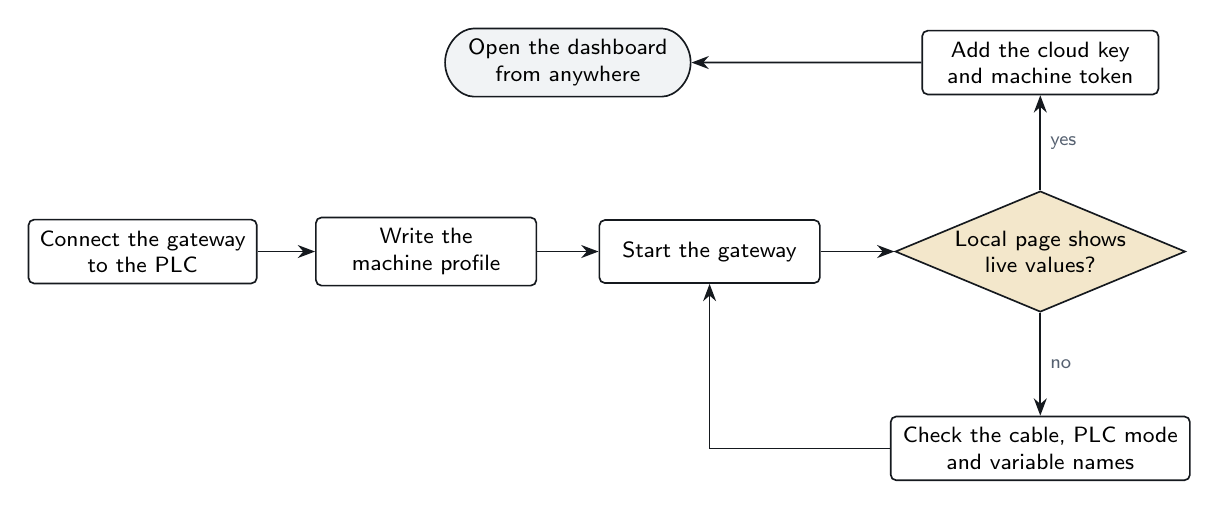
\begin{tikzpicture}[x=1cm,y=1cm]
  \node[proc,minimum width=28mm] (a) at (0,0) {Connect the gateway\\to the PLC};
  \node[proc,minimum width=28mm] (b) at (3.6,0) {Write the\\machine profile};
  \node[proc,minimum width=28mm] (c) at (7.2,0) {Start the gateway};
  \node[dec] (d) at (11.4,0) {Local page shows\\live values?};
  \node[proc,minimum width=38mm] (e) at (11.4,-2.5) {Check the cable, PLC mode\\and variable names};
  \node[proc,minimum width=30mm] (f) at (11.4,2.4) {Add the cloud key\\and machine token};
  \node[term,minimum width=34mm] (g) at (5.4,2.4) {Open the dashboard\\from anywhere};
  \draw[wire] (a) -- (b); \draw[wire] (b) -- (c); \draw[wire] (c) -- (d);
  \draw[wire] (d) -- node[right,note] {no} (e);
  \draw[wire] (e.west) -| (c.south);
  \draw[wire] (d) -- node[right,note] {yes} (f);
  \draw[wire] (f) -- (g);
\end{tikzpicture}
\caption{Onboarding. The local page at \code{http://localhost:8787} proves the PLC side before the cloud is involved.}
\end{figure}

\subsection{Describing your machine}\label{sec:profile}
A profile is one JSON file. It names the variables and gives each a label. No code changes are needed for a
new machine.
\begin{lstlisting}
{ "id": "press-2", "name": "Press 2", "probe": "PR_STEP",
  "vars":   { "step": "PR_STEP", "fault": "PR_FAULT", "running": "PR_RUNNING", "parts": "PR_COUNT" },
  "steps":  [ { "id": 0, "name": "Idle" }, { "id": 10, "name": "Clamp" } ],
  "faults": { "1": "Emergency stop pressed" },
  "inputs":  [ { "id": "DI-0", "label": "Guard closed", "var": "_IO_EM_DI_00" } ],
  "outputs": [ { "id": "DO-0", "label": "Clamp",        "var": "_IO_EM_DO_00" } ] }
\end{lstlisting}

\subsection{Reading the dashboard}
\begin{minipage}[t]{0.39\textwidth}\vspace{0pt}
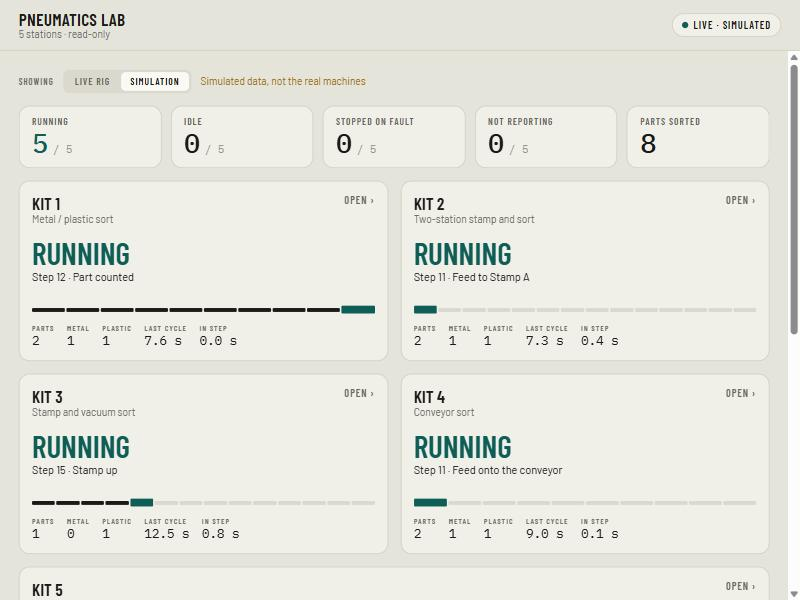
\includegraphics[width=\linewidth]{figures/floor.jpg}

{\small\color{sub}The floor view of the hosted app, here running its built-in simulation.}
\end{minipage}\hfill
\begin{minipage}[t]{0.55\textwidth}\vspace{0pt}
\begin{tabularx}{\linewidth}{@{}>{\raggedright\arraybackslash}p{30mm}Y@{}}
\toprule
\textbf{You see} & \textbf{It means} \\
\midrule
Running, Idle, Homing & The controller's own sequence state \\
Fault, with number and text & The program stopped itself; the Signals page shows which input is wrong \\
Stale, values dimmed & No new reading recently; values are the last known \\
PLC offline & The gateway runs but cannot reach the controller \\
No data & The gateway is not sending: computer off or no internet \\
Not connected & No controller is running that station's program \\
Simulated & Demonstration data generated in the app \\
\bottomrule
\end{tabularx}
\end{minipage}

\subsection{Security position}
\begin{tabularx}{\textwidth}{@{}>{\raggedright\arraybackslash}p{62mm}Y@{}}
\toprule
\textbf{Question} & \textbf{Answer today} \\
\midrule
Can this system start, stop or change my machine? & No. It implements reading only, at the protocol level and at the web API. \\
Does it open my plant network to the internet? & No. The gateway makes outbound HTTPS connections only. \\
Who can send data as my machine? & Only a holder of that machine's token. The cloud stores the token's hash, not the token. \\
Who can view my machine's state? & \gap\ Anyone who has the dashboard address. There is no sign-in yet. \\
Is history kept? & \gap\ No. Only the latest state is stored; the event log lives in the gateway's memory and resets when it restarts. \\
What happens if the internet drops? & \gap\ Readings in that period are not sent later. The local page keeps working. \\
\bottomrule
\end{tabularx}

% ------------------------------------------------------------------ 7
\section{Built versus proposed}
\begin{tabularx}{\textwidth}{@{}>{\raggedright\arraybackslash}p{62mm}lY@{}}
\toprule
\textbf{Capability} & \textbf{State} & \textbf{Evidence or next step} \\
\midrule
Read Micro850 tags by name, read-only & \built & Running against the rig; 24 to 28 ms per full scan \\
Automatic PLC discovery and reconnect & \built & Found the PLC again after its address changed \\
Program identification and profiles & \built & Kit 1, Kit 3 and an unknown-program fallback \\
Local API and live stream & \built & Checked; write methods refused \\
Cloud relay with token ingest & \built & Real PLC state seen in the hosted app; wrong token rejected \\
Dashboard: floor, station, signals, log, 3D & \built & Hosted; reported a real homing fault on 18 November \\
Unity twin live link & \built & Confirmed for Kit 1 \\
Twin and gateway reading at the same time & \gap & Each ran alongside CCW; not yet both together \\
Sign-in and per-user access & \gap & Required before wider sharing \\
History and trends & \prop & Time-series store in the cloud \\
Edge device, Linux packaging & \prop & Section~\ref{sec:edge} \\
Compact encoding, store and forward, MQTT & \prop & Section~\ref{sec:edge} \\
Commands from the app & \prop & Deliberately absent; only after sign-in, on a separate path \\
\bottomrule
\end{tabularx}

\vfill
{\scriptsize\color{sub}Product logos identify the technologies used or proposed and are trademarks of their owners; their use here does not imply endorsement.
Sources: \code{Tools/PlcGateway}, \code{Assets/Scripts/Runtime/PlcLink}, \code{Dashboard/}, and readings taken from the controller.
Diagrams are drawn with TikZ and charts with pgfplots.}

\end{document}
